%%%%%%%%%%%%%%%%%%%%%%%%%%%%%%%%%%%%%%%%%
% Masters/Doctoral Thesis 
% LaTeX Template
% Version 2.5 (27/8/17)
%
% This template was downloaded from:
% http://www.LaTeXTemplates.com
%
% Version 2.x major modifications by:
% Vel (vel@latextemplates.com)
%
% This template is based on a template by:
% Steve Gunn (http://users.ecs.soton.ac.uk/srg/softwaretools/document/templates/)
% Sunil Patel (http://www.sunilpatel.co.uk/thesis-template/)
%
% Template license:
% CC BY-NC-SA 3.0 (http://creativecommons.org/licenses/by-nc-sa/3.0/)
%
%%%%%%%%%%%%%%%%%%%%%%%%%%%%%%%%%%%%%%%%%

%----------------------------------------------------------------------------------------
%	PACKAGES AND OTHER DOCUMENT CONFIGURATIONS
%----------------------------------------------------------------------------------------

\documentclass[
11pt, % The default document font size, options: 10pt, 11pt, 12pt
%oneside, % Two side (alternating margins) for binding by default, uncomment to switch to one side
english, % ngerman for German
singlespacing, % Single line spacing, alternatives: onehalfspacing or doublespacing
%draft, % Uncomment to enable draft mode (no pictures, no links, overfull hboxes indicated)
%nolistspacing, % If the document is onehalfspacing or doublespacing, uncomment this to set spacing in lists to single
%liststotoc, % Uncomment to add the list of figures/tables/etc to the table of contents
%toctotoc, % Uncomment to add the main table of contents to the table of contents
%parskip, % Uncomment to add space between paragraphs
%nohyperref, % Uncomment to not load the hyperref package
headsepline, % Uncomment to get a line under the header
%chapterinoneline, % Uncomment to place the chapter title next to the number on one line
%consistentlayout, % Uncomment to change the layout of the declaration, abstract and acknowledgements pages to match the default layout
]{MastersDoctoralThesis} % The class file specifying the document structure

%\usepackage[utf8]{inputenc} % Required for inputting international characters
%\usepackage[T1]{fontenc} % Output font encoding for international characters

\usepackage{amssymb}
\usepackage[backend=bibtex,style=authoryear,natbib=true]{biblatex} % Use the bibtex backend with the authoryear citation style (which resembles \left( APA)

\addbibresource{example.bib} % The filename of the bibliography

\usepackage[autostyle=true]{csquotes} % Required to generate language-dependent quotes in the bibliography
\usepackage{import}
\usepackage{tikz}
\usepackage{tikz-network}
\usepackage{breqn}
\usepackage{bm}
\usepackage{graphicx}
\usepackage{subcaption}
\usepackage{multirow}
\usepackage{pdfpages}
\usepackage{rotating}
\usetikzlibrary{fit}
\usetikzlibrary{calc,patterns,angles,quotes}
\usetikzlibrary {arrows.meta,graphs,shapes.misc}
\usetikzlibrary {positioning}

\subimport{./layers/}{init}

\newcommand{\bn}{\textbf{n}}
\newcommand{\tabhead}[1]{\textbf{#1}}




\def\ConvColor{rgb:yellow,5;red,2.5;white,5}
\def\ConvReluColor{rgb:yellow,5;red,5;white,5}
\def\PoolColor{rgb:red,1;black,0.3}
\def\DcnvColor{rgb:blue,5;green,2.5;white,5}
\def\SoftmaxColor{rgb:magenta,5;black,7}
\def\SumColor{rgb:blue,5;green,15}
\def\poolsep{1}


%----------------------------------------------------------------------------------------
%	MARGIN SETTINGS
%----------------------------------------------------------------------------------------

\geometry{
	paper=a4paper, % Change to letterpaper for US letter
	inner=2.5cm, % Inner margin
	outer=3.8cm, % Outer margin
	bindingoffset=.5cm, % Binding offset
	top=1.5cm, % Top margin
	bottom=1.5cm, % Bottom margin
	%showframe, % Uncomment to show how the type block is set on the page
}

%----------------------------------------------------------------------------------------
%	THESIS INFORMATION
%----------------------------------------------------------------------------------------

\thesistitle{Improved Normal Inference from Calibrated Illuminated RGBD Images} % Your thesis title, this is used in the title and abstract, print it elsewhere with \ttitle
\supervisor{Prof. Dr. Didier \textsc{Stricker}}


 % Your supervisor's name, this is used in the title page, print it elsewhere with \supname
\examiner{} % Your examiner's name, this is not currently used anywhere in the template, print it elsewhere with \examname
\degree{Master of Science} % Your degree name, this is used in the title page and abstract, print it elsewhere with \degreename
\author{Jingyuan  \textsc{Sha}} % Your name, this is used in the title page and abstract, print it elsewhere with \authorname
\addresses{} % Your address, this is not currently used anywhere in the template, print it elsewhere with \addressname

\subject{Computer Science} % Your subject area, this is not currently used anywhere in the template, print it elsewhere with \subjectname
\keywords{} % Keywords for your thesis, this is not currently used anywhere in the template, print it elsewhere with \keywordnames
\university{\href{https://www.uni-kl.de/}{Technische Universität Kaiserslautern}} % Your university's name and URL, this is used in the title page and abstract, print it elsewhere with \univname
\department{\href{https://www.informatik.uni-kl.de/}{German Research Center for Artificial Intelligence}} % Your department's name and URL, this is used in the title page and abstract, print it elsewhere with \deptname
\group{\href{https://av.dfki.de/}{Augmented Vision}} % Your research group's name and URL, this is used in the title page, print it elsewhere with \groupname
\faculty{\href{http://faculty.university.com}{Faculty Name}} % Your faculty's name and URL, this is used in the title page and abstract, print it elsewhere with \facname

\AtBeginDocument{
\hypersetup{pdftitle=\ttitle} % Set the PDF's title to your title
\hypersetup{pdfauthor=\authorname} % Set the PDF's author to your name
\hypersetup{pdfkeywords=\keywordnames} % Set the PDF's keywords to your keywords
%\hypersetup{colorlinks=false}
\hypersetup{hidelinks}
}

\begin{document}

\frontmatter % Use roman page numbering style (i, ii, iii, iv...) for the pre-content pages

\pagestyle{plain} % Default to the plain heading style until the thesis style is called for the body content

%----------------------------------------------------------------------------------------
%	TITLE PAGE
%----------------------------------------------------------------------------------------

\begin{titlepage}
\begin{center}
\vspace*{.06\textheight}
{\scshape\LARGE \univname\par}\vspace{1.5cm} % University name
\textsc{\Large Master Thesis}\\[0.5cm] % Thesis type

\HRule \\[0.4cm] % Horizontal line
{\huge \bfseries \ttitle\par}\vspace{0.4cm} % Thesis title
\HRule \\[1.5cm] % Horizontal line
 
\begin{minipage}[t]{0.4\textwidth}
\begin{flushleft} \large
\emph{Author:}\\
\href{https://linkedin.com/in/jingyuan-sha-5b8b43208}{\authorname} % Author name - remove the \href bracket to remove the link
\end{flushleft}
\end{minipage}
\begin{minipage}[t]{0.4\textwidth}
\begin{flushright} \large
\emph{Supervisor:} \\
\href{https://av.dfki.de/members/stricker/}{\supname}\\
\href{https://av.dfki.de/members/fetzer/}{M. Sc. Torben \textsc{Fetzer}}
 % Supervisor name - remove the \href bracket to remove the link  
\end{flushright}
\end{minipage}\\[3cm]
 
\vfill


\groupname\\\deptname\\ % Research group name and department name
\includegraphics{Figures/TUK_LOGO_RGB}\\[2cm] % Research group name and department name
 
\vfill

{\large \today}\\[4cm] % Date
%\includegraphics{Logo} % University/department logo - uncomment to place it
 
\vfill
\end{center}
\end{titlepage}

%----------------------------------------------------------------------------------------
%	DECLARATION PAGE
%----------------------------------------------------------------------------------------

\begin{declaration}
\addchaptertocentry{\authorshipname} % Add the declaration to the table of contents
\noindent I, \authorname, declare that this thesis titled, \enquote{\ttitle} and the work presented in it are my own. I confirm that:

\begin{itemize} 
\item This work was done wholly or mainly while in candidature for a research degree at this University.
\item Where any part of this thesis has previously been submitted for a degree or any other qualification at this University or any other institution, this has been clearly stated.
\item Where I have consulted the published work of others, this is always clearly attributed.
\item Where I have quoted from the work of others, the source is always given. With the exception of such quotations, this thesis is entirely my own work.
\item I have acknowledged all main sources of help.
\item Where the thesis is based on work done by myself jointly with others, I have made clear exactly what was done by others and what I have contributed myself.\\
\end{itemize}
 
\noindent Signed:\\
\rule[0.5em]{25em}{0.5pt} % This prints a line for the signature
 
\noindent Date:\\
\rule[0.5em]{25em}{0.5pt} % This prints a line to write the date
\end{declaration}

\cleardoublepage

%----------------------------------------------------------------------------------------
%	QUOTATION PAGE
%----------------------------------------------------------------------------------------

\vspace*{0.2\textheight}

\noindent\enquote{\itshape Thanks to my solid academic training, today I can write hundreds of words on virtually any topic without possessing a shred of information, which is how I got a good job in journalism.}\bigbreak

\hfill Dave Barry

%----------------------------------------------------------------------------------------
%	ABSTRACT PAGE
%----------------------------------------------------------------------------------------

\begin{abstract}
\addchaptertocentry{\abstractname} % Add the abstract to the table of contents
The Thesis Abstract is written here (and usually kept to just this page). The page is kept centered vertically so can expand into the blank space above the title too\ldots
\end{abstract}

%----------------------------------------------------------------------------------------
%	ACKNOWLEDGEMENTS
%----------------------------------------------------------------------------------------

\begin{acknowledgements}
\addchaptertocentry{\acknowledgementname} % Add the acknowledgements to the table of contents
The acknowledgments and the people to thank go here, don't forget to include your project advisor\ldots
\end{acknowledgements}

%----------------------------------------------------------------------------------------
%	LIST OF CONTENTS/FIGURES/TABLES PAGES
%----------------------------------------------------------------------------------------

\tableofcontents % Prints the main table of contents

\listoffigures % Prints the list of figures

\listoftables % Prints the list of tables

%----------------------------------------------------------------------------------------
%	ABBREVIATIONS
%----------------------------------------------------------------------------------------

\begin{notations}{ll} % Include a list of abbreviations (a table of two columns)

\textbf{I} & Grayscale Image Matrix (Height $ \times $ Width $ \times $ 1)\\
\textbf{L} & Light Map Matrix (Height $ \times $ Width $ \times $ 3)\\
\textbf{N} & Normal Map Matrix (Height $ \times $ Width $ \times $ 3)\\
\textbf{V} & Vertex Map Matrix (Height $ \times $ Width $ \times $ 3)\\

\textbf{X} & Input Matrix (Height $ \times $ Width $ \times $ Channels)\\
\textbf{Y} & Output Matrix (Height $ \times $ Width $ \times $ Channels)\\

\textbf{w} & Width of Matrix\\
\textbf{h} & Height of Matrix\\



\end{notations}

%----------------------------------------------------------------------------------------
%	PHYSICAL CONSTANTS/OTHER DEFINITIONS
%----------------------------------------------------------------------------------------

\begin{constants}{lr@{${}={}$}l} % The list of physical constants is a three column table

% The \SI{}{} command is provided by the siunitx package, see its documentation for instructions on how to use it

Speed of Light & $c_{0}$ & \SI{2.99792458e8}{\meter\per\second} (exact)\\
%Constant Name & $Symbol$ & $Constant Value$ with units\\

\end{constants}

%----------------------------------------------------------------------------------------
%	SYMBOLS
%----------------------------------------------------------------------------------------

\begin{operations}{ll} % Include a list of Symbols (a three column table)

$[A B]$ & concatenation between A and B \\
$\oplus$ & element-wise multiplication \\
$\cdot$ & dot product \\
%Symbol & Name & Unit \\

\addlinespace % Gap to separate the Roman symbols from the Greek

$\omega$ & angular frequency & \si{\radian} \\

\end{operations}

%----------------------------------------------------------------------------------------
%	DEDICATION
%----------------------------------------------------------------------------------------

\dedicatory{To ...} 

%----------------------------------------------------------------------------------------
%	THESIS CONTENT - CHAPTERS
%----------------------------------------------------------------------------------------

\mainmatter % Begin numeric (1,2,3...) page numbering

\pagestyle{thesis} % Return the page headers back to the "thesis" style

% Include the chapters of the thesis as separate files from the Chapters folder
% Uncomment the lines as you write the chapters

% Chapter Template

\chapter{Introduction} % Main chapter title

\label{ch:introduction} % Change X to a consecutive number; for referencing this chapter elsewhere, use \ref{ChapterX}

%----------------------------------------------------------------------------------------
%	SECTION 1
%----------------------------------------------------------------------------------------

\section{From 3D to 2D}

\section{Kinect and Surface Normal}

As a popular and affordable new type of depth sensor, Kinect, had attracted a great focus to computer vision research in the last decades. It simultaneously captured the grayscale or RGB image and depth map with a high resolution. The depth map can further convert to structured point clouds with known intrinsic calibration parameters, which can use in many applications.

%% why surface normal is important
Surface Normal is one of the most worthy pieces of information that can infer from point clouds, which applies in many practical applications, such as augmented reality and robotics. Some tasks like shading and surface reconstruction require normal as one of the inputs. However, due to the lack of accuracy of the sensors, the  surface normal inference from depth maps/point clouds has many challenges.  


%-----------------------------------
%	SUBSECTION 1
%-----------------------------------
\section{Standard Methods}

%%%%%%%%%%%%%%%%%%% talk about the reason of this thesis %%%%%%%%%%%%%%%%%%

%% standard method for normal inference is insufficient, input is sparse, not robust enough
Standard methods compute normals from the point cloud using neighboring information in image space or from a single grayscale image using use Shape from Shading \cite{SFS}. The first method assumes that the neighbors of the points locate on the same plane. This method performs well with a well-chosen window size. However, the drawbacks are that the algorithm is highly noise sensitive. It is weak in handling missing pixels, which is a common issue in the input data. The second method depends on the correct information about the light source. Errors may occur in regions with inter-reflections in the 3D measurement. 

%-----------------------------------
%	SUBSECTION 2
%-----------------------------------

\section{Deep Learning based Method}
%% CNN based methods
Recently, deep learning based method \cite{yolov3}, \cite{efficientDet} achieved a great succeed for image processing. 
These network architectures use a batch of RGB/Grayscale images as input and usually employ for classification problems. Usually, the images are convoluted with a convolutional layer and downsampling with pooling layers. The outputs of the network consist of a single value to represent the index of the corresponding class \cite{efficientDet}, or with a set of values to represent the position of bounding boxes.\cite{yolov3}.  

However, in many other vision tasks, like normal map inference, the output is demanded as the same shape as the input. Instead of predicting one or several classes for the whole input matrix, the class for each pixel requires for prediction. In this case, the traditional network architecture is not suitable anymore.


%----------------------------------------------------------------------------------------
%	SECTION 2
%----------------------------------------------------------------------------------------

\section{Challenges of Normal Inference}

%% talk about upsampling 
Recently, deep learning-based methods are used in computer vision tasks such as image segmentation, image inpainting, and depth density enhancement. In these methods, multiple architectures have proposed with an upsampling section. In this case, the output can be designed to have the same shape as the input or slightly smaller. Nevertheless, the resolution is similar to the input image. The normal Inference task has a similar pipeline compared to these tasks.


%% there exists space for improvement 
On the other hand, the point cloud data provided by Kinect or similar RGB-D, and LiDAR sensors are only semi-dense. A huge amount of missing pixels distribute all over the images, and some of the regions leave complete empty holes. This situation imposes another challenge on normal inference. 

The depth image is incomplete, however, the depth sensor is able to capture grayscale texture images, which are typically fully dense due to their passive nature. Furthermore, if the texture image is already illuminated by strong directional light of a video projector, whose position is known, then there should exist theoretical relations between light direction, normal direction, and grayscale image. Then the normal can be inferred better using the given image information and depth map.  Based on the grayscale image and corresponding semi-dense depth maps, a CNN model can be designed to infer the normal map, which can give more density and robust results comparing to the standard algorithm. 


%% add noise image
\begin{figure}[th]
	\centering
	\includegraphics[width=.4\textwidth]{Figures/kinect-depth.png}
	\decoRule
	\caption{A captured depth map via infrared sensors. Pixels that far away represent by light colors, otherwise by dark colors. The black dots are the depths that failed to be detected.}
\label{fig:kinect-depth}
\end{figure}


%% add noise image

\begin{figure}[th]
	\centering
	\includegraphics[width=.4\textwidth]{Figures/real-normal.png}
	\decoRule
	\caption{Semi-dense Normal Map calculated from depth map using a standard method}
\label{fig:standard-normal-inference}
\end{figure}


%%%%%%%%%%%%%%%%%% talk about the main work in this thesis  %%%%%%%%%%%%%%%%%%
\section{Main Works of this thesis}
In this thesis, we found a solution for the problems mentioned above and proposed a novel deep learning architecture for surface normal inference. A network named Albedo Gated Normal Inference Network(AlGaN) is proposed to infer normal given the corresponding depth map. The architecture of AlGaN involves a two-stage CNN. The first stage infers the normal map using point cloud as input. If the light source position and grayscale image can be provided further, the second stage infers the albedo altogether with the normals from the first stage. In addition, the loss function is based on least-square error and Lambertian reflection.

With the help of synthetic data in Unity, a dataset is created for CNN model training. It can provide accurate ground truth for training work, which real data is usually not provided. The results of this dataset show that our AlGaN model performs also well on real data captured by Infrared cameras. The trained Normal models achieve a remarkably better prediction accuracy at a low computational cost compared to the standard approaches for semi-dense point clouds. 
% Chapter Template

\chapter{Related Work} % Main chapter title

\label{ch:02} % Change X to a consecutive number; for referencing this chapter elsewhere, use \ref{ChapterX}




%% depth map approach
Surface normal inference is a widely researched topic and can be solved in multiple directions. Based on a structured point cloud, the surface normal can be derived from geometry information of the point cloud, which mainly utilizes the neighbor information and consider it as an optimization problem (\cite{optimized-methods} ). They can perform well on dense point cloud input data based on a well-chosen window size. However, the drawbacks are that the algorithms are highly noise sensitive. 
The point cloud is usually not fully dense and normally converted from depth map, which are usually with missing pixels and holes on dark, shinny or transparent regions (\cite{nyu}). The missing points destabilizes the geometry based solution. To ease this problem, \cite{Holzer.S} proposed method to use local neighbors with an interest parameter $ p $ and compute the eigenvectors of the corresponding covariance matrix, which is used to smooth the depth data in order to handle the noise of depth image.  \cite{depth-inpainting-distribution} proposed an approach considers the depth distributions of neighboring regions to fill the holes in the depth map. 
Some approaches use deep learning method to fill missing areas. \cite{nconv} introduces normalized convolution to deal with missing or uncertain depth data with an added mask on the standard convolution operation. \cite{ncnn} applied it and use it as normalized convolution layers in their networks, which aims to reconstruct the missing pixels from the sparse depth map sensed by cameras. \cite{pncnn} proposed an input confidence estimation network to estimate the confidence instead of using a binary mask.


%% photometric approach
Photometric stereo is another approach that infer surface normal from BRDF based surface model. The surface normal is related with observed intensity, the incoming light direction, the outgoing viewing direction and the light intensity. It required multiple light conditions to get an optimal solution. 







%% fusion approach


%% talk about gated convolution, Unet

%% in summary

\paragraph{Unstructured Point Cloud Based}
For the unstructured point cloud, the neighbor information of each point is usually unknown. K-nearest neighbor (KNN) is a common algorithm for neighbor searching. With knowing this information, the neighbor based approaches can be used as a second step. However, KNN-method merely based on the Euclidean distance in the 3D space. Therefore, the points of the other surfaces but in a close distance will also be considered as neighbors. To ease this problem, \cite{unstructed-pc} proposed a method based on unstructured point cloud with selecting the optimal scale around each point for normal estimation. To calculate the normals of multiple points in parallel \cite{unstructed-pc-patch-stitching} processes a series of overlapping patches for normal estimation. 



Deep learning based methods take single RGB image or RGB-D image as the input for normal estimation. It has a strong relationship with the depth inference tasks, two benchmarks are highly used in these area. (\cite{nyu} and \cite{kitti-depth}) Based on the input of training model, the methods can be roughly divided as follows: 



\paragraph{RGB based} RGB based methods predict the depth map diretly from single RGB image.
\cite{Eigen} proposed a two staged network for depth map prediction based on RGB image, which consider the global features and the local features respectively. \cite{img2depth} employed Residual Network for the feature extraction and further designed a upsampling part which replace the fully-connected layer with the unpolling layers. 
\cite{geometry_based_solution} proposed a method to learn discriminative and geometrically informative primitives from RGBD images, which is further used to recover the surface normals of a scene from a single image. 
\cite{GeoNet} uses ResNet (\cite{resnet}) to infer a coarse surface normal based on RGB image, and further refine it with the help of depth map based on the methods based on \cite{geometry_based_solution}. \cite{binsformer} proposed a method achieved state of art in NYUv2 Dataset (\cite{nyu}), which adaptively generate information to predict depth maps based on RGB image.

\paragraph{RGB-D based}
\cite{hfm} based on UNet architecture for normal estimation using RGB-D image as input. The RGB image and depth map are in the separate branches and imply a fusion module in four sections of the network to concatenate two branches. It also considers the confidence of the values in depth map.

\cite{depth-enhance-guided} further integrated RGB image as the guidance to deal with the missing pixels in the depth map. 








 
% Chapter Template
\chapter{Approaches} % Main chapter title

\label{ch:03} %

The normal inference task involves estimating the surface normal of a 3D object, assuming that the surface of the object is mathematically unknown. This means that we cannot simply use the cross product of two non-parallel surface vectors to find the normal. Instead, the surface is sensed by digital sensors under certain types of data, which can be divided into two groups. The first group is geometry data, where a point cloud is used to capture the geometry information of the surface in 3D space. The approach that uses point clouds for normal estimation is called geometry-based approach.
Another type of data is images that record the reflectance and shading of the surface under the following lighting conditions. The surface normal is calculated based on specific light models such as BRDF. The other approach, which uses the relationship between reflectance and shading to calculate the surface normal, is called photometric stereo.

In this chapter, the geometric and photometric stereo based approaches are presented separately. Then, a method for estimating the surface normal using both types of data based on deep learning approaches is introduced.





\section{Notations}

In the following chapters of this thesis the following standard notations are used. The bold capital letters stand for matrices, while the bold lowercase letters stand for vectors. The Greek capital letters stand for planes.
The subscript $ i= \{1,2,...\} $ stands for the index of observations, the superscript for the dimension of the matrices or vectors, e.g. $ \textbf{n}^{3\times 1} $ for a vector of dimension $ 3\times 1 $. We use $ W $ for the width, $ H $ for the height and $ C $ for the number of channels.


\section{Geometry-based Normal Estimation}

Geometry-based normal estimation uses the point cloud of the object surface as input. The task can be formulated as follows.

Given a structured point cloud $ \textbf{V}^{W\times H\times 3} $, in which the 3D point positions are stored with respect to the image grid. We want to compute the corresponding normal map $ \textbf{N}^{W\times H \times 3} $. The normal map is simply a matrix representation of the normals of all points in the point cloud. A normal $ \textbf{n}^{3\times 1} $ at the point $ \textbf{p}^{3\times 1} \in \textbf{V} $ is a unit vector whose direction is outward from the surface and perpendicular to the tangent plane of the surface at point $ \textbf{p} $.


The idea behind the neighborhood-based method is to fit a plane $ \tilde\Pi $ containing the $ k $ neighbors $ \textbf{p}_1, ..., \textbf{p}_k \in \mathbb{R}^{3\times1} $ of the point $ \textbf{p} $, then compute the normal $ \tilde{\textbf{n}} $ of the plane $ \tilde\Pi $. The $ \tilde{\textbf{n}} $ is considered as an approximation to the normal $ \textbf{n} $ of the tangent plane $ \Pi $.

The point and its neighbors are assumed to lie in the same plane $ \Pi $, which is exactly the tangent plane of the surface at the point $\textbf{p} $. 
This is usually not true for most of the surface, since the surface is usually not flat, but has some degree of curvature. But if $ k $ is of a suitable scale and the point cloud is dense enough, we can approximately consider all $ k $ neighboring points in a small area on the same tangent plane. Then we have an approximation $ \textbf{n} \approx \tilde{\textbf{n}}$, where $ \tilde{\textbf{n}}$ denotes the estimated normal. Similarly, the estimated tangent plane $ \tilde{\Pi} \approx \Pi $. 


Based on the above assumption, the task of normal inference is trivial, since the surface is then mathematically describable. We can generate the approximate tangent plane at each point with its neighbors, then the normal $ \tilde{\textbf{n}} $ of the tangent plane can be derived from the following equations.

\[\tilde{\textbf{n}} \cdot \textbf{v}_{ij} = 0 \]
where 
\[ \textbf{v}_{ij} = \textbf{p}_i - \textbf{p}_j, \text{for } i, j \in \{ 1,2,...,k\}, i\neq j \]
To find a normal, we need at least 3 neighbors that are not on the same line to solve the above equation. Calculate the normal for each point on the point cloud, then we can get the corresponding normal maps. 

If we consider more than 3 neighbors, the points are usually not on the same plane. In this case, the system of equations is overdetermined. We can use the optimization approach to find a plane that has the least distance to all points in 3D space. By $ \textbf{A }\in \mathbb{R}^{k\times 3} $ we denote the vector matrix vertically stacked by the $ k $ vectors we found on the approximated tangent surface. Then the system of equations is transformed into an optimization problem 



\begin{equation}
	\begin{array}{rrclcl}
		\displaystyle \min & \multicolumn{3}{l}{\|\textbf{ A}  \bn \|^2_2} \\
		\\
		\textrm{s.t.} & \| \bn \|^2_2 & = & 1 
	\end{array}
\end{equation}
where the additional condition is added to avoid trivial solutions, and the normal is supposed to be a unit vector.

The above problem can be solved by singular value decomposition (SVD), where.
\[ \textbf{A}= \textbf{U}\boldmath{\Sigma} \textbf{V}^T \]
The last column of $ \textbf{V} $ is the solution of the system of equations and consequently the surface normal. 

The optimization based approach using SVD is more robust compared to selecting only 3 points for normal computation, since the plane generated by 3 neighbors is not guaranteed to be a good approximation to the actual tangent plane. However, the size of the neighbors $ k $ is a key parameter of this approach. For the smooth surface, a relatively larger $ k $ can help the system of equations find a plane that is closer to the tangent plane. For the sharp surface, $ k $ must be small enough to ensure that the points it contains are still approximately in the same plane, otherwise the more points it contains will just be the outliers for the equation solution. 

Finally, after solving the above equation, we should convert all normals to the viewpoint $ \textbf{s} $ for uniformity. Thus, the direction of a normal should be inverted if 


\begin{equation}\label{eq:normal-invertion}
	\textbf{n} \cdot (\textbf{p}  - \textbf{s}) > 0
\end{equation}
Since the above approach is essentially solved by SVD, this method will be referred to as \textit{SVD} in the remainder of the paper for simplicity.

\section{Photometric Stereo based Normal Estimation}
Photometric stereo was originally introduced by \cite{photometric-stereo} and is a completely different approach from the geometry information based approach such as \textit{SVD}. It estimates the surface normal of the object by observing the object in the same position under different illuminated conditions. It is based on the fact that the light reflected from a surface depends on the surface normal and the light direction.

Before presenting this approach, let us discuss what we can actually obtain from the images.
An image $ \textbf{I} $ can be decomposed into two parts: the reflectance $ \textbf{R} $ and the shading $ \textbf{S} $,
\[ \textbf{I} = \textbf{R}\odot \textbf{S}\]
where $ \odot $ denotes the element-wise product. This decomposition of the image is based on the intrinsic image model proposed by \cite{intrinsic-image}. It interprets the observed image into a reflection image and a shading image. Figure \ref{fig:intrinsic-image} shows a visualization of the decomposition.

%% insert an image for decompositions
\begin{figure}[th]
	\centering
	\captionsetup{width=\linewidth}
	{\includegraphics[width=.19\textwidth]{./Figures/intrinsic_image.png}}
	{\includegraphics[width=.19\textwidth]{./Figures/intrinsic_image_reflectance.png}}
	{\includegraphics[width=.19\textwidth]{./Figures/intrinsic_image_shading.png}}
	{\includegraphics[width=.19\textwidth]{./Figures/intrinsic_image_light.png}}
	{\includegraphics[width=.19\textwidth]{./Figures/intrinsic_image_normal.png}}
	\decoRule
	\caption{Intrinsic image analysis of the Washington object. From left to right: original image, reflection image, shading image, light image, normal image.}
	\label{fig:intrinsic-image}
	
\end{figure}

The equation can be further decomposed based on different surface models. If we assume that the object surfaces are Lambertian surfaces, i.e. surfaces that reflect light in all directions, as shown in Figure \ref{fig:lambertian-surface}, then the reflectance is equal to the albedo $ \rho $, the shading image can be decomposed as the product of the radiance of the incident light $ L_0 $ and the cosine of the angle of incidence, which is the dot product of the surface normal $ \textbf{N} $ and the light source direction $ \textbf{L} $.
\[ \textbf{I} = \rho \odot ( L_0 \textbf{L} \cdot \textbf{N}) \]
Note that each surface normal in the matrix $ \textbf{N} $ and each light direction in the matrix $ \textbf{L} $ is a unit vector, so they have only two degrees of freedom. 


\begin{figure}[th]
	\centering
	\captionsetup{width=\linewidth}
	\begin{subfigure}[b]{0.49\linewidth}
		\includegraphics[width=\textwidth]{./Figures/Lambertian-Reflection-Lambertian-Surface.png}
	\end{subfigure}
	\begin{subfigure}[b]{0.49\linewidth}
		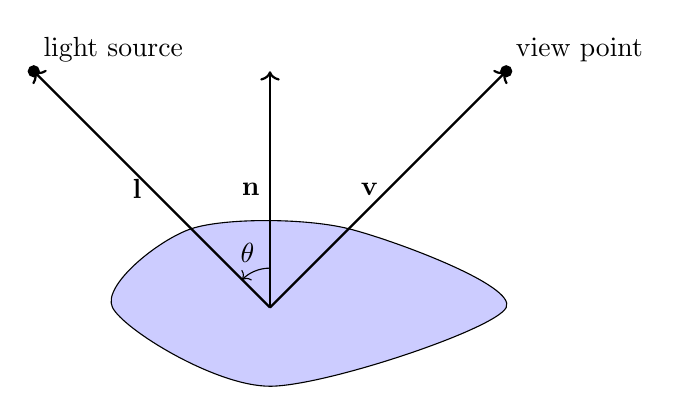
\begin{tikzpicture} 
			% reference lines
			\coordinate (light) at (-1,3);
			\coordinate (p) at (2,0);
			\coordinate (normal) at (2,3);
			\draw [fill=blue!20] plot [smooth cycle] coordinates {(0,0) (1,1) (3,1) (5,0) (2,-1)}; %% surface element
			\draw[thick, ->] (2,0) -- (2,3) node[midway, left] {$ \textbf{n} $}; %% normal
			\draw[thick, ->] (2,0) -- (-1,3) node[midway, left] {$ \textbf{l} $}  ; %% source direction
			\pic [draw, ->, "$\theta$", angle eccentricity=1.5] {angle = normal--p--light};
			\draw[thick, ->] (2,0) -- (5,3) node[midway, left] {$ \textbf{v} $}; %% view direction
			\filldraw[black] (-1,3) circle (2pt) node[anchor=south west]{light source}; %% light source
			\filldraw[black] (5,3) circle (2pt) node[anchor=south west]{view point}; %% view point		
		\end{tikzpicture}
	\end{subfigure}
	\decoRule
	\caption{Left: the reflection of light on a Lambertian surface. (Image source \cite{lambertian-reflectance}). Right: the surface normal, the light direction of the source and the viewing direction, where $ \theta $ denotes the angle between the light direction and the normal.}
	\label{fig:lambertian-surface}
\end{figure}
The equation can be rearranged as follows
\[ \textbf{I} =(L_0\rho \odot \textbf{N}) \cdot ( \textbf{L}) \]
Let $ \textbf{G} =L_0\rho \odot \textbf{N} $, the equation simplifies to
\[\textbf{I} = \textbf{G} \cdot \textbf{L}\]
If we use a set of $ k $ images for the same scene, taken based on different light projections. Then, for each pixel $ (x,y) $ in a scene, we can set up a system of equations 

\[ 
\begin{pmatrix}
	\textbf{l}_1^T \\
	\textbf{l}_2^T \\
	\cdots \\
	\textbf{l}_k^T
\end{pmatrix} \textbf{G}(x,y) = 
\begin{pmatrix}
	\textbf{I}_1(x,y) \\
	\textbf{I}_2(x,y) \\
	\cdots \\
	\textbf{I}_k(x,y)
\end{pmatrix}
\]
For simplicity, $ \textbf{l}_i^T $ for $ 1\le i \le k $ denotes the direction of light at position $ (x,y) $ in $ k $-th image . The equation can be solved using the least squares method. Then, the albedo can be determined with the light intensity, since the normal is a unit vector,

\[ \| \textbf{G}(x,y)\|_2 = \|L_0\rho(x,y)\textbf{N}(x,y)\|_2 = L_0\rho(x,y) \]
Then the normal can be determined as follows

\[ \textbf{N}(x,y) = \frac{\textbf{G}(x,y)}{L_0\rho(x,y)}\]
We compute the surface normal for each point to obtain the surface normal map. 

This approach is also called Shape from Shading (\textit{SFS}) \cite{SFS}. Both normal maps and the corresponding albedo are obtained from a series of images under different lighting conditions. Since the direction of light is used in the calculation, the cameras and the position of the light source must be calibrated beforehand. 

In the shape from shading approach, at least three light positions are considered for normal estimation on a pixel. It is also common to use more than three light sources to cover most points of the surface as much as possible. 

We assume that in each neighborhood there is a coherent behavior for the albedo that can be modeled by the filters in the neural network, and in the following section we propose an learning based approach for normal inference from geometry information, but using only one illuminated scene.


\newpage 
\section{Gated Convolution Neural Network for Surface Normal Estimation}
\label{sec:gcnn}

Recently, Deep Learning based methods have achieved great success in image processing\cite{yolov3} \cite{efficientDet}. These network architectures use a stack of RGB/grayscale images as input and are used for classification problems. Typically, the images are convolved with convolutional layers and sampled with pooling layers. The output values of the networks consist of a single value representing the index of the corresponding class, or a set of values representing the position of the bounding boxes\cite{yolov3}. However, in many other image processing tasks, such as inference of normal maps, the output is required to have the same form as the input, while each pixel in the output image requires a prediction. Therefore, the output consists not only of one or several labels, but of a matrix similar in size to the input. In this case, the traditional network architecture with full connections in the last layers is no longer suitable for label prediction.

%% talk about image upsampling, unet
\cite{unet} has proposed an architecture called \textit{U-Net} for biomedical image segmentation. The architecture is shown in Figure \ref{fig:u-net}. This net has a very regular architecture for data processing, while the down/up sampling part has a similar design. For the feature extraction part, called down-sampling, the architecture follows the traditional CNN architecture. For the up-sampling part, the network uses an architecture similar to the down-sampling operations, which uses the same convolutional operations but replaces the max-pool layers with up-conv layers. An important design is the skip connection in the up-sampling part. The feature maps extracted in the down-sampling part are concatenated with the feature maps in the up-sampling part. This helps the network to find the locations in the original image and use them to predict a sharp output.

\begin{figure}[th]
	\centering
	\captionsetup{width=\linewidth}
	\includegraphics[width=\textwidth]{./Figures/u-net-illustration-correct-scale2.pdf}
	\decoRule
	\caption{The structure of UNet. (Image source:\cite{unet})}
	\label{fig:u-net}
\end{figure}

% why we need a mask
The \textit{U-Net} relies on standard convolutional layers to construct the network. This is useful for image processing tasks with fully dense input data, since there are no missing pixels.
However, for some other input data, such as depth maps acquired by light scanners, it is not always fully dense data, but data with many missing pixels and holes. In this case, we can still apply the standard convolutional layers to extract the feature maps from the semi-dense depth map, but then the valid pixels and the invalid pixels (the missing pixels) will be mixed up during training, resulting in blur and color discrepancy as mentioned by \cite{partial_conv}. Therefore, it is useful to find a way to distinguish the valid and invalid pixels during training. 

\cite{pncnn0} use a binary mask to denote valid pixels, and also use normalized convolution as a surrogate for the default convolutional layer in the training model. The normalized convolution is represented as follows

\begin{equation}
	\begin{array}{rrclcl}
		O(x,y) = 
		\begin{cases}
			\dfrac{\Sigma_i^k\Sigma_j^k W(i,j) \odot I(x-i,y-j) \odot M(x-i,y-j)}{\Sigma_i^k\Sigma_j^k W(i,j) \odot M(x-i,y-j)}, & \text{if}\ \sum_{i}^k\sum_{j}^k M(i,j)>0 \\
			0, & \text{otherwise}
		\end{cases}
	\end{array}
\end{equation}
where $ k $ is the kernel size, $ (x,y) $ is the position in the input, $ (i,j) $ is the displacement in the kennel, and $ M $ is the corresponding mask. A binary mask uses 1 to indicate valid pixels, and 0 otherwise. $ \odot $ denotes element-wise multiplication.



\subsection{Gated Convolution}

% introduce gconv
\cite{gated_activation} proposed a gated activation unit to model more complex interactions compared to standard CNN layers. This was mainly inspired by the multiplicative units that exist in the Long Short-Term Memory (\textit{LSTM}) proposed by \cite{lstm} and the Rated Recurrent Unit (\textit{GRU}) proposed by \cite{gru}. \cite{gconv} has deployed the same gated unit and uses it as a gated convolution layer for training tasks with incomplete input data, such as image inpainting tasks. In this gated convolution layer, the mask used to distinguish between valid and invalid pixels is not specified in advance, but learned during training. The advantage is that the erroneous measurements that are not masked in the depth data can be learned during training to further improve performance. 

The structure is shown in Figure \ref{fig:gconvLayer}. Instead of using a mask as input to indicate valid pixels, a standard convolutional layer is used to learn this mask directly from the data, and a sigmoid function is used as an activation function to indicate the confidence of pixel validation. Meanwhile, another standard convolutional layer is set aside to learn the feature maps with a ReLU/LeakyReLU activation function. Therefore, both the mask and the input features are learned during training.  Then, an element-wise multiplication is performed with the feature map and the mask as the final feature map of this gated convolution layer. 

Formally, the gated convolution is described as follows: the layer with the input $ (N, C_{in}, H, W) $ and the output $ (N, C_{out}, H_{out}, W_{out}) $:

\begin{equation}\label{gconv}
	o(N_i, C_{o_j}) = \sigma(\sum_{k=0}^{C_{in}-1}w_g(C_{o_j}, k) \star i(N_i,k) + b_g(C_{o_j})) * 
	\phi (\sum_{k=0}^{C_{in}-1}w_f(C_{o_j}, k) \star i(N_i,k) + b_f(C_{o_j}))
\end{equation}
where $ \phi $ is the LeakyReLU function, $ \sigma $ is the sigmoid function, so the output values are in the range $ [0,1] $. $ \star $ is the valid 2D cross-correlation operator, $ N $ is the batch size, $ C $ denotes the number of channels, $ H $ is the height of the input planes in pixels, and $ W $ is the width in pixels, $ w(C_{o_j},k) $ denotes the weight of the $ j $-th output channel corresponding to the $ k $-th input channel, $ i(N_i, k) $ denotes the input of the $ i $-th stack corresponding to the $ k $-th input channel, $ b(C_{o_j}) $ denotes the bias of the $ j $-th output channel.


% Gated Convolution Layer
\begin{figure}[H]
	\centering
	\captionsetup{width=\linewidth}
	\begin{tikzpicture}
		\tikzstyle{rect} = [rectangle, rounded corners, minimum width=2.5cm, minimum height=1cm,text centered, draw=black, fill=blue!20]
		\tikzstyle{arrow} = [thick,->,>=stealth]
		\node (output) [rect] {Output};
		\node (oplus) [below of=output, yshift=-.2cm] {$\Huge\odot $};
		\node (LeakyReLU) [rect,below of=oplus, yshift=-0.3cm] {Feature};
		\node (sigmoid) [rect, below of=oplus, yshift=-0.3cm, xshift=-3cm] {Gating};
		
		\node (conv1) [rect,below of=sigmoid, yshift=-1cm] {Gating};
		\node (conv2) [rect,below of=LeakyReLU, yshift=-1cm] {Feature};
		\node (input) [below of=oplus] at (0,-7) {\includegraphics[width=.25\textwidth]{./Figures/train-input.png}};
		
		\draw [arrow] (oplus) -- (output);
		\draw [arrow] (sigmoid) |- (oplus);
		\draw [arrow] (LeakyReLU) -- (oplus);
		
		\draw [arrow] (conv2) --  node [text width=2.5cm, midway, right=1em]{LeakyReLU} (LeakyReLU);
		\draw [arrow] (conv1) --  node [text width=2.5cm, midway, right=1em]{Sigmoid} (sigmoid);
		\draw [arrow] (input) -|  node [text width=2.5cm, midway, below=1em]{Conv2D} (conv1);
		\draw [arrow] (input) -- node [text width=2.5cm, midway, right=1em]{Conv2D} (conv2);
		
		
		
		\node (conv-output) [rect, ] at (6,0) {Output};
		\node (conv-LeakyReLU) [rect,below of=conv-output, yshift=-0.4cm] {Feature};
		\node (conv-conv2) [rect,below of=conv-LeakyReLU, yshift=-1cm] {Feature};
		\node (conv-input) [below of=conv-output] at (6,-7) {\includegraphics[width=.25\textwidth]{./Figures/train-input.png}};
		
		\draw [arrow] (conv-LeakyReLU) -- (conv-output);
		
		\draw [arrow] (conv-conv2) --  node [text width=2.5cm, midway, right=1em]{LeakyReLU} (conv-LeakyReLU);
		\draw [arrow] (conv-input) -- node [text width=2.5cm, midway, right=1em]{Conv2D} (conv-conv2);
		
		
		
	\end{tikzpicture}
	\decoRule
	\caption{Left: Gated Convolution Layer, where $ \odot $ denotes element-wise multiplication. Right: standard convolution layer.}
	\label{fig:gconvLayer}
\end{figure}


%\section{Canny Edge Detection for Detail Enhancement}
%The inaccuracy part is usually concentrate in the coarse surface or drastic changed surface parts of the object. The corresponding part can be extracted separately via edge detector algorithms, like Canny Edge detector. Feed the edges to a special net for normal prediction might improve the accuracy further. 

\subsection{GCNN Architecture}
\label{sec:architecture}

Based on the above implementation, we proposed a network based on the \textit{U-Net} proposed by \cite{unet}, replacing the standard convolutional layers with gated convolutional layers used for semi-dense normal inference tasks, called gated convolution neural network (\textit{GCNN}), as shown in Figure \ref{fig:gcnn-archi}. 

\begin{sidewaysfigure}[h]
	\centering
	\captionsetup{width=\linewidth}
	\includegraphics[width=\textwidth]{Figures/gcnn}
	\decoRule
	\caption{The architecture of Gated convolution neural network (\textit{GCNN}) based on Gated convolution and \textit{U-Net} Architecture.}
	\label{fig:gcnn-archi}
\end{sidewaysfigure}

To describe the network in a uniform way, the parameters of the network are represented by letters.
The network consists of a downsampling part and an upsampling part. In the downsampling part, the input has the form $ \textbf{X}_{in} \in \mathbb{R}^{H\times W\times C_{in}}$, while the output is of the form $ \textbf{X}_{out} \in \mathbb{R}^{H\times W\times C_{out}}$
The input matrix goes through 3 down-samples. A down-sampling block consists of two gated convolution layers with stride (1,1) and an additional gated convolution layer with stride (2,2) to reduce the resolution of the feature map. Thus, there are a total of 3 gated convolution layers in each downsampling operation.
The total of three downsamplings extract the geometry features $ \textbf{X}_f $ from the input matrix $ \textbf{X}_{in} $ (represented as regression function $ f $)
\[ f: \textbf{X}_{in} \rightarrow X_f \]
After feature extraction, the network upsamples the feature map three times to obtain the output matrix $ \textbf{X}_{out} $. Each upsampling consists of an interpolation operation that uses nearest neighbor interpolation for upsampling the feature map, and a concatenation layer that concatenates the interpolated result and the corresponding high-resolution feature map $ \textbf{X}_{df_1}, \textbf{X}_{df_2}, \textbf{X}_{df_3} $ from the downsampling part. This is also called a skip connection. In the last step, a gated convolution layer is used to reduce the channel size to fit the next upsampling block. After upsampling three times, the resolution goes back to the original size. After that, two standard convolutional layers without activation function are added to predict the surface normals. The entire upsampling branch can be represented as a regression function $ n $,
\[ n: \textbf{X}_f, \textbf{X}_{df_1}, \textbf{X}_{df_2}, \textbf{X}_{df_3} \rightarrow \textbf{X}_{out} \]
All convolutional layers of the network use the same kernel size $ 3\times 3 $. 


One of the main features of the network is that the output has the same size as the input. This is achieved by (1,1) padding and the same number of channels in the convolution layers. Thus, the surface normal map can be estimated with the same dimension as input data. Another important point of the network is its robustness to noise using gated convolutional layers. The network can take a semi-dense matrix as input and then predict the fully dense matrix as output. The last feature is the multipurpose use of scenarios. No specific input type is given in the description. 
The network is also fully convolutional and therefore can accept different input resolutions. 


\section{Illuminated Calibrated RGB-D Image based Normal Inference}
\label{sec:trip-net}
The GCNN architecture is designed for one type of input, since it has only one pipe to process the data. In our work, the input refers to a structured point cloud. Therefore, it is suitable for a geometry-based approach that uses the point cloud as input and estimates the corresponding surface normal. However, as mentioned in the introduction, the goal of this work is to discuss the improvement of normal inference based on an illuminated calibrated RGB-D image, i.e., we want to see if we can improve the performance of normal estimation not only based on geometry information such as the point cloud or the depth map, but also with illumination information such as the image and the light map. Therefore, we need to find an architecture that takes into account all these types of data. 


\subsection{Light Map, Gray-scale Image and Vertex Map}
\label{sec:lightmap}
First, we present the required input types for our network.

\paragraph{Vertex Map}
The vertex map $ \textbf{V} $ is converted from the depth map presented in chapter \ref{ch:04}, while the depth map is acquired from a depth camera. It contains a set of surface point locations in 3D space. Each pixel in the vertex map corresponds to a point position. These vertices contain the geometry information of the object surface, which can be further used for training deep learning models. For each scene, the camera takes only one image, leaving only one vertex map. However, as mentioned earlier, the vertex map is only semi-dense. We use such a semi-dense vertex map as input for the surface normal estimation.

\paragraph{Grayscale Image}
The grayscale image $ \textbf{I} $ is acquired in correspondence with the depth map using the same calibrated camera equipment, so the intrinsic matrix $ \textbf{K} $ and the extrinsic camera matrix $ [\textbf{R}|\textbf{t}] $ are known. Unlike the vertex map, it is usually completely dense.

\paragraph{Light Map}
The light map $ \textbf{L} $ can be derived from the vertex map $ \textbf{V} $. The position of the light source $ (s_x, s_y, s_z) $ is given by the input data. As shown in Figure \ref{fig:lambertian-surface}, the direction of the incident light is a vector point from the light source to the surface point and can therefore be calculated as follows.

\begin{equation}\label{light-direction}
	\begin{array}{ll}
		\textbf{L}(x,y,z)&= \dfrac{\textbf{V}(x,y,z)-(s_x,s_y, s_z)}{\|\textbf{V}(x,y,z)-(s_x,s_y, s_z)\|_2}\\ 
	\end{array}
\end{equation}
where both $ (s_x, s_y, s_z) $ and $ \textbf{V} $ refer to the camera space. The light direction map $ \textbf{L} $ is normalized since only the direction of the light is considered. Applying the above equation for all pixels in the point cloud, we obtain the corresponding light map, which is a matrix with the same size as the point clouds. However, it should be noted that the light map is calculated based on the vertex map, while the vertex map in the training pipeline is only semi-dense, so the light map is also semi-dense and has the same noise feature as the vertex map, as shown in Figure \ref{fig:light-input}. 

\begin{figure}[H]
	\centering
	\captionsetup{width=\linewidth}
	{\includegraphics[width=.32\textwidth]{./Figures/intrinsic_image_vertex_input.png}}
	{\includegraphics[width=.32\textwidth]{./Figures/intrinsic_image_light_input.png}}
	{\includegraphics[width=.32\textwidth]{./Figures/intrinsic_image.png}}
	\decoRule
	\caption{Three kinds of input data. From left to right, vertex map, light map, gray-scale image.}
	\label{fig:light-input}
\end{figure}
See chapter \ref{ch:04} for more details on how to set up the dataset.


%\subsection{VIL Net}
%Based on above implementations, we propose a light and image guided network called Vertex-Image-Light Network (VIL-Net). The structure is basically derived from GCNN model as mentioned in \ref{sec:gcnn}, which is shown in Figure 
%\ref{fig:VIL-Net}.
%
%As mentioned in the name, the \textbf{VIL}-Net utilizes \textbf{V}ertex map, \textbf{L}ight map and \textbf{I}mage map to accomplish the normal inference task. 
%
%The network can be consider in two parts. The first part extracts the feature maps from the input data. It deals with two kinds of input, the vertex map $ X_1 \in \mathbb{R}^{w\times h\times3}$, and the concatenation of light and image map $ X_2 \in \mathbb{R}^{w\times h\times4} $. The network extracts the geometry features $ X_v $ from vertex map $ X_1 $ (represented as a regression function v)
%\[ v: X_1 \rightarrow X_v \]
%and the photometric features $ X_l $ from image and the light map $ X_2 $ (represented as a regression function $ l $)
%\[ l: X_2 \rightarrow X_l \]
%where the two encoders have the same network architecture based on the downsampling part of GCNN model. After the feature extraction, 2 extra layers are added: 1, a concatenate layer is added to fuse the vertex feature, and the image and light map feature getting from the encoder. 
%2, a fused feature map is predicted from all the feature maps base on a single gated convolution layer. (represented as a regression function $ m $)
%\[ m: [X_v X_l] \rightarrow X_f \]
%Then the network interpolates the feature maps $ X_f $ 3 times using interpolation and gated convolution layers to inference the normal map $ N $. Meanwhile, the skip connections fuse the high resolution features $ X_{df_1, df_2, ...} $ from the downsampling part during the upsamplings. The upsampling is represented as a regression function $ n $:
%\[ n: X_f, X_{df_1, df_2, ...} \rightarrow N \]
%
%With the help of an extra image-light encoder, the network gained more information of the object surface, which is supposed to predict the surface normal more accurate. In this scenario, the output is still the surface normal, thus the training loss can be the same as GCNN model.


\subsection{Trip-Net Architecture}
We proposed a network that considers the vertex map, the light map, and the grayscale image for surface normal inference, which is called the Triple-Pipe-Gated Network (\textit{Trip-Net}). 
The \textit{Trip-Net} uses the GCNN architecture three times to perform the normal inference task, so we call it \textit{Triple-Pipe-Gated}. The architecture is shown in Figure \ref{fig:Trip-Net}.

The network consists of three pipes combined with one main pipe and two side pipes. Each pipe deals with a different task. The Main Pipe deals with the geometry information, which takes the vertex map as input and is used to predict the surface normal. The light map takes a Side Pipe as input, from which the light features are extracted and then passed to the Main Pipe as additional information for normal estimation. The image map takes another Side Pipe to extract the image features, and then forwards the features to the Main Pipe as well. The additional pipes provide the illumination information that helps the Main Pipe refine the inferred normals.

\paragraph{Side-Pipe (Light)}
 The structure of the Light-Pipe is almost identical to the architecture of the GCNN. It takes the light map $ \textbf{L} \in \mathbb{R}^{W\times H\times 3}$ as input and then passes through gated convolution layers three times to obtain the feature maps,
 $ \textbf{X}_{L1D} \in \mathbb{R}^{{W}\times H\times C} $,
 which has the same resolution as the input map.
 Then three downsampling operations are followed afterwards. In each downsampling, 3 gated convolution layers are used to further extract the feature maps, where the first two gated convolution layers have stride (1,1) and the third gated convolution layer has stride (2,2). Then we get
  
$ \textbf{X}_{L2D} \in \mathbb{R}^{\frac{W}{2}\times \frac{H}{2}\times C} $,
$ \textbf{X}_{L3D} \in \mathbb{R}^{\frac{W}{4}\times \frac{H}{4}\times C} $,
$ \textbf{X}_{L4D} \in \mathbb{R}^{\frac{W}{8}\times \frac{H}{8}\times C} $
(represented as a regression function $ l_{down} $)
\[ l_{down}: \textbf{L} \rightarrow  \textbf{X}_{L1D} , \textbf{X}_{L2D}, \textbf{X}_{L3D}, \textbf{X}_{L4D} \]
For the up-sampling operation, it takes 3 times up-sampling to generate higher resolution light feature maps
$ \textbf{X}_{L1U} \in \mathbb{R}^{{W}\times {H}\times C} $,
$ \textbf{X}_{L2U} \in \mathbb{R}^{\frac{W}{2}\times \frac{H}{2}\times C} $,
$ \textbf{X}_{L3U} \in \mathbb{R}^{\frac{W}{4}\times \frac{H}{4}\times C} $ respectively, whereas each up-sampling also considers the feature maps in the down-sampling part,
(represented as a regression function $ l_{up1}, l_{up2}, l_{up3} $)
\[ 
\begin{matrix}
	l_{up3} : \textbf{X}_{L3D}, \textbf{X}_{L4D} \rightarrow \textbf{X}_{L3U} \\
	l_{up2} : \textbf{X}_{L2D}, \textbf{X}_{L3U} \rightarrow \textbf{X}_{L2U} \\
	l_{up1} : \textbf{X}_{L1D}, \textbf{X}_{L2U} \rightarrow \textbf{X}_{L1U} \\
\end{matrix}
\]
In our network, each up-sampling is done in three layers, an interpolation layer based on the nearest neighbor algorithm, a concatenation layer to concatenate the interpolated feature maps and the corresponding feature maps in the down-sampling part, and a gated convolution layer to reduce the channel size.
The light pipe branch is completed in the last layer of the third up-sampling.

In this branch, four kinds of feature maps $ \textbf{X}_{L4D}, \textbf{X}_{L3U}, \textbf{X}_{L2U}, \textbf{X}_{L1U} $ are used as guided information for further operation.

\paragraph{Side-Pipe (Image)}

The task of the Image-Pipe in the network is to predict the image features. This pipe is a pipe cooperating with the Light-Pipe. The architect is the same as that of the Light-Pipe, but only the input is the image matrix $ \textbf{I}\in \mathbb{R}^{W\times H\times 1}$. The first set of the feature maps are $ \textbf{X}_{I1D} \in \mathbb{R}^{{W}\times H\times C} $, noting that it has the same channel as the light feature maps. Then, the down-sampling is performed three times to extract the image feature maps

$ \textbf{X}_{I2D} \in \mathbb{R}^{\frac{W}{2}\times \frac{H}{2}\times C} $,
$ \textbf{X}_{I3D} \in \mathbb{R}^{\frac{W}{4}\times \frac{H}{4}\times C} $,
$ \textbf{X}_{I4D} \in \mathbb{R}^{\frac{W}{8}\times \frac{H}{8}\times C} $
(represented as a regression function $ i_{down} $)
\[ l_{down}: \textbf{I} \rightarrow  \textbf{X}_{I1D} , \textbf{X}_{I2D}, \textbf{X}_{I3D}, \textbf{X}_{I4D} \]
It requires three times upsampling to produce higher resolution image feature maps.
$ \textbf{X}_{I1U} \in \mathbb{R}^{{W}\times {H}\times C} $,
$ \textbf{X}_{I2U} \in \mathbb{R}^{\frac{W}{2}\times \frac{H}{2}\times C} $,
$ \textbf{X}_{I3U} \in \mathbb{R}^{\frac{W}{4}\times \frac{H}{4}\times C} $ respectively, whereas each up-sampling also considers the feature maps in the down-sampling part,
(represented as a regression function $ i_{up1}, i_{up2}, i_{up3} $)
\[ 
\begin{matrix}
	i_{up3} : \textbf{X}_{I3D}, \textbf{X}_{I4D} \rightarrow \textbf{X}_{I3U} \\
	i_{up2} : \textbf{X}_{I2D}, \textbf{X}_{I3U} \rightarrow \textbf{X}_{I2U} \\
	i_{up1} : \textbf{X}_{I1D}, \textbf{X}_{I2U} \rightarrow \textbf{X}_{I1U} \\
\end{matrix}
\]
whereas the layers in the upsampling part have the same architecture as the Light Pipe. In the Image Pipe, four types of feature maps $ \textbf{X}_{I4D}, \textbf{X}_{I3U}, \textbf{X}_{I2U}, \textbf{X}_{I1U} $ are used as guided information for further operation.


\paragraph{Main-Pipe (Vertex)}
The task of the vertex pipe in the network is to predict the normal map directly, also taking into account the feature maps in the other channels. The input is the vertex map $ \textbf{V} \in \mathbb{R}^{W\times H\times 3}$ converted from the point cloud. 
The downsampling part is still the same as for the other two pipes. The feature maps in each downsampling part are of the form
$ \textbf{X}_{V1D} \in \mathbb{R}^{{W}\times H\times C} $, 
$ \textbf{X}_{V2D} \in \mathbb{R}^{\frac{W}{2}\times \frac{H}{2}\times C} $,
$ \textbf{X}_{V3D} \in \mathbb{R}^{\frac{W}{4}\times \frac{H}{4}\times C} $,
$ \textbf{X}_{V4D} \in \mathbb{R}^{\frac{W}{8}\times \frac{H}{8}\times C} $, respectively, 
(represented as a regression function $ i_{down} $)
\[ v_{down}: \textbf{V} \rightarrow  \textbf{X}_{V1D} , \textbf{X}_{V2D}, \textbf{X}_{V3D}, \textbf{X}_{V4D} \]
The up-sampling operation has a different situation than the other two pipes.
It merges the output feature maps with the corresponding resolution from three pipes to get a merged feature map 
$ \textbf{X}_{F3U} \in \mathbb{R}^{W\times H\times C} $, 
$\textbf{X}_{F2U} \in \mathbb{R}^{W\times H\times C} $, 
$\textbf{X}_{F1U} \in \mathbb{R}^{W\times H\times C} $,
in each up-sampling stage, (represented as regression functions $ f_{up1}, f_{up2}, f_{up3}, f_{up4}$)
\[ 
\begin{matrix}
	f_{up4} : \textbf{X}_{I4D}, \textbf{X}_{L4D}, \textbf{X}_{V4D} \rightarrow \textbf{X}_{F4U} \\
	f_{up3} : \textbf{X}_{I3U}, \textbf{X}_{L3U}, \textbf{X}_{F4U} \rightarrow \textbf{X}_{F3U} \\
	f_{up2} : \textbf{X}_{I2U}, \textbf{X}_{L2U}, \textbf{X}_{F3U} \rightarrow \textbf{X}_{F2U} \\
	f_{up1} : \textbf{X}_{I1U}, \textbf{X}_{L1U}, \textbf{X}_{F2U} \rightarrow \textbf{X}_{F1U} \\
			
\end{matrix}
\]
Each upsampling consists of 5 layers: An interpolation layer to double the resolution using the nearest interpolation algorithm, a gated layer to reduce the channel size to 1/3 of itself for inter-pipes feature reduction, a concatenation layer to connect the output with the corresponding feature map in the downsampling part (skip connection), a gated layer to reduce the channel size to 1/2 of itself for skip-connection feature reduction, a concatenation layer to merge the corresponding upsampling feature map from the other two pipes with the feature map in the current pipe altogether. These 5 layers take into account both the information from the other pipes and the feature maps from the downsampling part. 

At the end of the network, to fit the task of normal inference, two standard convolutional layers are added to convert the normal map $ \textbf{X}_{N} \in \mathbb{R}^{\frac{W}{8}\times \frac{H}{8}\times 3} $ (represented as a regression function $ n $)
\[n:\textbf{X}_{F1U} \rightarrow \textbf{X}_{N} \] 

\begin{sidewaysfigure}[h]
	\centering
	\captionsetup{width=\linewidth}
	\includegraphics[width=\textwidth]{Figures/trignet} % Research group name and department name
	\decoRule
	\caption{The architecture of the \textit{Trip-Net}.}
	\label{fig:Trip-Net}
\end{sidewaysfigure}



%% loss function 

\subsection{Loss Functions}
We have investigated different loss functions for training our network. The most common loss functions are the L1 loss and the L2 loss for image simulation. In our experiments, we used a modified Huber loss function to train our model, which yields a lower error in the evaluation compared to a pure L1 or L2 loss function. 

\paragraph{L1 Loss}
L1 loss, also known as absolute error loss, which calculates the absolute difference between the prediction and the ground truth. It leads to the mean value of the absolute errors of the observations.
\[ L_1(\tilde y - y) = |\tilde y - y | \]

\paragraph{L2 Loss}
The standard loss function for optimization in regression problems is the L2 loss, also known as squared error loss, which minimize the squared difference between a prediction and the actual value. It leads to the mean of the observations. 
\[ L_2(\tilde y - y) = \|\tilde y - y \|_2^2 \]


%\paragraph{Masked L2 Loss with penalty for outliers(mask-l2)}
%\label{par:maskl2}
%The background pixels of the input data are not considered in the normal inference task, they are saved as black pixels in the input data. These pixels should not considered in the loss function, i.e. invalid pixels. Therefore, a valid mask is required to distinguish the background and the main object. Specifically, using a matrix with the same width and height as the output, for each pixel, 0 is invalid, 1 is valid. 
%Furthermore, depends on the specific task, the output should be constraint in a range. For normal output, the range is $ [-1,1] $. Thus for the outliers out of this range, a outlier mask can be applied to give them a penalty.
%
%\begin{equation}\label{gcnn-loss}
%	\begin{array}{ll}
%		l(x,y)&= L  = \{l_1, ..., l_N\}^T\\ 
%		l_{n\in N} &= \| mask_{obj} \odot mask_{ol} \odot ( {\tilde y}_n - y_n) \|_2^2 + 	\| mask_{obj} \odot mask_{nol} \odot ( {\tilde y}_n - y_n) \|_2^2 \\
%	\end{array}
%\end{equation}
%
%where $ x $ is input, $ y $ is target, $ N $ is the batch size.$ mask_{obj} $ is the mask of the object, i.e. 1 means it is an pixel on the object, 0 is an pixel on the background. $ mask_{ol} $ is the mask for the outliers, i.e. 1 means outliers, 0 means non outlier, $ mask_{nol} $ is exactly the inverse of $ mask_{ol} $. $ p $ is the penalty of the outliers, it is set as 1.4.


\paragraph{Huber Loss}
Inspired by \cite{img2depth}, we use the Huber loss provided by \cite{berhu-loss} for our model training, which indeed achieves a better error than a simple L2 loss. It can be described mathematically as follows.


\begin{equation}\label{berhu-loss}
	\begin{array}{ll}
		\mathcal{B}(y)= \begin{cases}
			|y| & |y| \ge c \\
			\dfrac{y^2 + c^2}{2c} & |x| < c\\
		\end{cases}
	\end{array}
\end{equation}
where $ c=0.2\max (|\tilde y - y|) $. The shape of the loss is shown in Figure \ref{fig:berhu-loss-shape}. Huber loss is a combination of L1 and L2 loss, being L2 loss in the range $ [-c,c] $ and L1 loss outside this range. The loss is also differentiable at the junction of two first order intersection functions. As mentioned in \cite{img2depth}, the parameter $ c=0.2 \max(|\tilde y - y|) $ corresponds to the 20\% of the maximum error per batch. 

\begin{figure}[H]
	\centering
	\captionsetup{width=\linewidth}
	\begin{tikzpicture}
		\pgfplotsset{ticks=none}
		\begin{axis} [axis lines=center]
			\addplot [domain=1:2, smooth, thick, width=5mm, color=red] { x };
			\addplot [domain=0:1, smooth, width=5mm] { x };
			\addplot [domain=-1:0, smooth, width=3mm] { -x };
			\addplot [domain=-2:-1, smooth, thick, width=3mm, color=red] { -x };
			\addplot [domain=-1:0, smooth, thick, color=red] { (x^2+1^2)/(2*1) };
			\addplot [domain=0:1, smooth, thick, color=red] { (x^2+1^2)/(2*1) };
		\end{axis}
	\end{tikzpicture}
	\caption{The shape of Huber Loss (show in red line). }
	\label{fig:berhu-loss-shape}
\end{figure}



% Chapter Template

\chapter{Dataset} % Main chapter title

\label{ch:04} % Change X to a consecutive number; for referencing this chapter elsewhere, use \ref{ChapterX}

%----------------------------------------------------------------------------------------
%	SECTION 1
%----------------------------------------------------------------------------------------

In this work, we need two types of input data to train our models. 
First, we need to know the geometry of the object surface. This can be captured by a depth camera, which records the distance of the object surface from the optical center of the camera and can be converted into a point cloud. 
Second, we need information about the illumination of the object surface, which is used as photometric information for further improvements. 
This type of information requires an observed image of the object with the light directions projected onto the object surface. 

To obtain this data, we can use a structured light scanner to scan the objects in the laboratory. However, the scanner usually cannot scan the dark, shiny, and transparent areas, resulting in many missing pixels and holes in the depth map. This incomplete surface information makes it difficult to train our model because the ground truth corresponding to the depth map is also incomplete. Second, training a deep learning-based model usually requires a large dataset, especially for a network without a backbone. Creating a single deep map dataset for this work would require too much work and resources. A suitable way to obtain huge depth map data with illumination information is to use a game engine that can simulate an arbitrary number of data.

We use the Unity game engine for data generation. Using a $ C\# $ script, we can set up a similar configuration in the lab. We then create a dataset based on the collected objects. The dataset we created for this work is called \textit{synthetic-50-5} because it contains 50 different object models for training and 5 object models for testing.

\section{Data Resources}
The object models we used were collected from the Internet.
A number of point cloud datasets for image processing research have been published by \cite{data1}, \cite{data2}, \cite{data3}, and \cite{data4}. Some of these point clouds were scanned from real objects using high-resolution scanners such as the Cyberware 3030 MS+ and calibrated with post-processing. These objects were scanned hundreds of times, fully capturing the original objects with up to millions of points\cite{data1}. Some of them are fully digitally synthesized. The dense point clouds make the normal inference task trivial, as the neighborhood-based method works adequately for this type of task. Some of the point clouds even contain precomputed normal maps based on more advanced methods. They all provide the accurate ground truth for the supervised learning method.

The \textit{synthetic-50-5} is a dataset we created in this work based on 50 point clouds as the training set and 5 point clouds as the test set. In creating the dataset, we tried to use as many object types as possible to cover a robust and wide range of training scenarios. There are several categories of models, such as figurines, animals, statues, toys, furniture, antiques, and car models, some of which have relatively smooth surfaces, such as model \textit{arm, bus, rabbit, cat, zebra}, and some of which have very intricate details, such as model \textit{Washington, Car-Engine, Armadillo}. 
We created this dataset for normal inference tasks. Figure \ref{fig:dataset-demo} shows illustrations of some objects. Appendix \ref{AppendixA} contains a complete version of the models of the dataset.


\begin{figure}[!h]
	\centering
	\captionsetup{width=\linewidth}
	\begin{subfigure}[b]{0.24\linewidth}
		\includegraphics[width=\linewidth]{./Figures/train-dataset/00.apoll.png}
		\caption{apoll}
	\end{subfigure}
	\begin{subfigure}[b]{0.24\linewidth}
		\includegraphics[width=\linewidth]{./Figures/train-dataset/01.arm.png}
		\caption{arm}
	\end{subfigure}
	\begin{subfigure}[b]{0.24\linewidth}
		\includegraphics[width=\linewidth]{./Figures/train-dataset/02.armadillo.png}
		\caption{armadillo}
	\end{subfigure}
	\begin{subfigure}[b]{0.24\linewidth}
		\includegraphics[width=\linewidth]{./Figures/train-dataset/03.bearded-guy.png}
		\caption{bearded-guy}
	\end{subfigure}
	
	\begin{subfigure}[b]{0.24\linewidth}
		\includegraphics[width=\linewidth]{./Figures/train-dataset/08.pergolesi-side-chair_texture.png}
		\caption{chair}
	\end{subfigure}
	\begin{subfigure}[b]{0.24\linewidth}
		\includegraphics[width=\linewidth]{./Figures/train-dataset/42.zebra_texture.png}
		\caption{zebra}
	\end{subfigure}
	\begin{subfigure}[b]{0.24\linewidth}
		\includegraphics[width=\linewidth]{./Figures/test-dataset/01.bus_texture.png}
		\caption{bus}
	\end{subfigure}
	\begin{subfigure}[b]{0.24\linewidth}
		\includegraphics[width=\linewidth]{./Figures/test-dataset/03.baoshanlu_texture.png}
		\caption{baoshanlu}
	\end{subfigure}
	\decoRule
	\caption{Some of the objects used for \textit{Synthetic-50-5}}
	\label{fig:dataset-demo}
\end{figure}
In addition, some objects also have colored textures, as shown in the second line of Figure \ref{fig:dataset-demo}. This is specifically prepared for the illuminated approach, since the image is used to evaluate the surface normals. By using textured models, our models get closer to the real dataset and have improved robustness that can be further applied to the real dataset.



\definecolor{direction-light-color}{RGB}{255,244,214}
\newcommand{\col}[1]{%
	\textcolor{#1}{\vrule width 0.5cm}}
\section{Synthesizing Scenes using Unity}

To simulate the data acquisition scenario as realistically as possible. We made the following settings. A flat cylinder, called \textit{stage} , is placed in the center of the 3D space as a platform for placing objects. We fixed the \textit{stage} in a predetermined position that will not be changed when images are captured. 
A directional light with RGB color FFF4D6 \col{direction-light-color} is placed 25 m away in the top view direction as an ambient light, which also has a fixed position.
An RGB-D camera is placed about 10 m away from the stage in the top-view direction. The camera captures the depth map and the grayscale image, which are randomly arranged after each scene. The movement range of the camera is 0.1 m in both directions of the X, Y and Z axes and a randomly changed Euler angle of $ 1^\circ $. 
A point light is placed about 5 m away as the illumination light, which is also moved randomly after each scene. The range of motion is 0.3 m in both directions of the X, Y and Z axes and $ 1^\circ $ randomly in the Euler angle.

During data acquisition, the object is randomly selected and placed on the stage. The object has a random rotation of up to $ 30^\circ $ in the $roll $ axis direction, a $ 30^\circ $ rotation in the $pitch $ axis direction, and a $ 180^\circ $ degree rotation in the $yaw $ axis direction. This gives the camera the ability to capture most directions of the objects. The layout in the Unity game engine is shown in Figure \ref{fig:unity-workplace}. We generate 3000 scenes with resolution $ 128\times128 $ and 5000 scenes with resolution $ 512\times512 $.

\begin{figure}[h!]
	\centering
		\captionsetup{width=\linewidth}
	\includegraphics[width=\linewidth]{./Figures/unity-workplace.PNG}
	\decoRule
	\caption{The layout of synthetic scene generation in Unity.}
	\label{fig:unity-workplace}
\end{figure}
The main advantage of generated scenes is the availability of complete information. We can capture the depth map in a lossless way. The corresponding normal map can also be safely considered as ground truth. And the scale of the dataset is easy to control. Table \ref{tab:data-files} gives more dataset information.
\begin{table}
	\centering
	\begin{tabular}{l l}
		\toprule
		\tabhead{Data} & \tabhead{Size} \\
		\midrule
		Depth map & Width$ \times $Height$ \times $ 1 \\
		\hline 
		Depth range  & MinDepth, MaxDepth \\  
		\hline
		Grayscale Image	&  Width$ \times $Height$ \times $ 1 \\  
		\hline 
		Normal Map &   Width$ \times $Height$ \times $ 3  \\
		\hline 
		Light Position &  $ 3\times1 $  \\
		\hline
		Camera Intrinsic Matrix &  $ 3\times 3 $  \\
		\hline 
		Camera Extrinsic Matrix &  $ 3\times 4 $  \\
		\bottomrule
	\end{tabular}
	\caption{The information saved for each scene in \textit{synthetic-50-5}.}
	\label{tab:data-files}
\end{table}


A critical detail we need to pay attention to is the exposure of the camera. Or we need to control the light emission on the object surface. As can be seen in Figure \ref{fig:camera_exposure}, too much exposure causes the surface texture to be difficult to see, resulting in clipping. In our experiments, we found that an appropriate light setting is essential for the illumination-based approach. Too much or too little lighting effects do not improve the illumination-based approach.

\begin{figure}[H]
	\centering
	\captionsetup{width=\linewidth}
	\begin{subfigure}[b]{0.32\linewidth}
		\includegraphics[width=\textwidth]{./Figures/wrong_exposure_2.png}
		\caption{Insufficient light}
	\end{subfigure}
	\begin{subfigure}[b]{0.32\linewidth}
		\includegraphics[width=\textwidth]{./Figures/right_exposure.png}
		\caption{Just Right}
	\end{subfigure}
	\begin{subfigure}[b]{0.32\linewidth}
		\includegraphics[width=\textwidth]{./Figures/wrong_exposure.png}
		\caption{Too much light}
	\end{subfigure}
	\decoRule
	\caption{Different exposure to the objects.}
	\label{fig:camera_exposure}
\end{figure}




\section{Data Preprocessing}
The raw data collected by Unity required further processing before it could be fed into the training models. 
\paragraph{Depth Map}
A depth map is a 1-channel image that contains information about the distance from the object surface to the camera center. It is stored as a 16-bit grayscale image, meaning that each pixel is in the range $\mathtt{0 - 65535}$. 

The raw depth maps in real data acquired by light scanners usually have missing pixels. To achieve a good match to the real data, a uniformly distributed noise was added to the synthetic data to randomly remove the valid pixels in the depth maps.
The simulated noise is uniformly distributed over the entire map with a certain noise intensity. A parameter $ \mu $ is used to control the intensity of the noise. It specifies the $ \mu $ pixel drop in percent. For example, at $ \mu-10 $, 10\% of the pixels are randomly removed. For each scene, the noise operation is based on a random $ \mu $ in a range $ \left[0, 50\right] $. In some scenes there are more missing pixels, in others less. The random noise intensity also allows the model to learn scenarios not only with noise, but also with low noise or even no noise.
Figure \ref{fig:noise-intensity} shows the noise effect at different $ \mu $.



%% add noise image
\begin{figure}[!h]
	\centering
	\captionsetup{width=\linewidth}
	{\includegraphics[width=\textwidth]{./Figures/add_noise_depth.png}}
	\decoRule
	\caption{From left to right: Noise-intensity on $ \mu-0$, $\mu-10$, $\mu-20$, $\mu-30$, $\mu-40$, $\mu-50$. Object Name: \textit{elephant-zun-lid}.}
	\label{fig:noise-intensity}
\end{figure}

%\begin{figure}[h!]
%	\centering
%	\begin{tikzpicture} 
%		% reference lines
%		\node[inner sep=10pt] (input) at (0,0)
%		{\includegraphics[width=\linewidth]{./Figures/ply_config.png}};
%		
%		%		\draw[thick,dashed]	(0,0) -- (10,0) ; % bottom
%		%		\draw[thick,dashed]	(0,3) -- (10,3) node[pos=0.9, above] {image plane}; % middle
%		%		\draw[thick,dashed]	(0,6) -- (10,6); % top
%		% camera 
%		%		\filldraw[black] (5,0) circle (2pt) node[anchor=south west]{Camera Position};
%		% world point 
%		%		\filldraw[black] (2,2) circle (2pt) node[anchor=north west]{Point};
%		% image point
%		%		\filldraw[black] (6,3) circle (2pt) node[anchor=north west]{Pixel};
%		% similiar triangles
%		%		\draw[thick] (0,0) -- (2,6); % AB
%		%		\draw[thick] (5,0) -- (7,6); % AC
%		%		\draw[thick] (5,6) -- (7,6) node[midway, below] {$ X $}; % BC
%		%		\draw[thick] (5,3) -- (6,3) node[midway, below] {$ u $};
%		%		% measure arrows
%		%		\draw[thick, <->] (4,0) -- (4,3) node[midway, left] {$ fk_u $};
%		%		\draw[thick, <->] (3,0) -- (3,6) node[pos=0.3, left] {$ Z $};
%	\end{tikzpicture}	
%	\caption{Data Collection configuration}
%	\label{fig:depth-triangulation}
%\end{figure}
The depth map is converted to a 3D vertex map after adding the noise.
Consider a 3-dimensional Euclidean space. The $ X $ and $ Y $ axes are perpendicular to each other align with the direction of width and height of the depth map separately. The $ Z $ axis is point inward (i.e., from view point to the depth map). The depth provided in the depth map is the distance from camera center to the object surface. Thus, in order to find the corresponding 3D vertex map $ \textbf{V}_C $ with respect to the camera coordinate system, we only need to multiple the depth matrix $ \textbf{Depth} $ with the point direction matrix $ \textbf{Dir} $.

\begin{dgroup*}
	\begin{dmath*}
		\textbf{V}_C = \textbf{Depth} \odot \textbf{Dir}
	\end{dmath*}
\end{dgroup*}

For the direction $ \textbf{Dir}(x,y,z) $ of a point $ \textbf{V}(x,y,z) $, it's X and Y components can be mapped from the corresponding pixel position $ (u,v) $ on the depth map, whereas the Z component is the focal length $ fk $ in pixels. Then we have to further normalize it to an unit vector.

\begin{dgroup*}
	
	\begin{dmath*}
		\textbf{Dir}(x, y, z) = \dfrac{(u, v, fk)}{\|(u, v, fk) \|_2}
	\end{dmath*}

\end{dgroup*}
Conversion of a point from the camera coordinate system to the world coordinate system using the extrinsic matrix $ R $ and $ t $
\[\textbf{V}_W = \textbf{V}_C R+t \]


%% How to represent input tensor, to make it fast converse
The sizes of the individual training objects are different. We normalized them to a unit scale so that they have a relatively similar distance from the camera.
In Figure \ref{fig:data_range} we have plotted the variations in value in each axis before normalization. Table \ref{tab:data_range} gives a quantitative evaluation of the corresponding average values. 

The normalization was performed as follows. First, the points are translated to the original point as much as possible, then the range value of an axis is chosen as the scaling factor, and the points are normalized to unit vectors. The equation is represented as follows

\begin{dgroup*}
	\begin{dmath*}
		X_n =\frac{X-\min(X)}{s}
	\end{dmath*}
	\begin{dmath*}
		Y_n = \frac{Y-\min(Y)}{s}
	\end{dmath*}
	
	\begin{dmath*}
		Z_n = \frac{Z-\min(Z)}{s}
	\end{dmath*}
	\begin{dmath*}
		s = \max(X)-\min(X)
	\end{dmath*}
\end{dgroup*}
where $ s $ is a scaling factor calculated as the range of the $ X $ axis, but theoretically it can also be the range of $ Y $ or $ Z $ axis.


\begin{figure}[!h]
	\centering
	\captionsetup{width=\linewidth}
	\begin{subfigure}[b]{0.49\linewidth}
		\includegraphics[width=\textwidth]{./Figures/Data_Extreme.png}
		\caption{Extreme Values in each axis }
	\end{subfigure}
	\begin{subfigure}[b]{0.49\linewidth}
		\includegraphics[width=\textwidth]{./Figures/Data_Range.png}
		\caption{Vertex Range in each axis}
	\end{subfigure}
	\decoRule
	\caption{The position fluctuation of the points in 100 Vertex Maps. 
		Left: Extreme values in 3 axes; Right: Vertex range in 3 axis.}
	\label{fig:data_range}
\end{figure}

\begin{table}[th]
	\centering
	\captionsetup{width=\linewidth}
	\begin{tabular}{c | c c c}
		\toprule
		\tabhead{Axis} & \tabhead{Scale} & \tabhead{Min} & \tabhead{Max}\\
		\midrule
		X & 1.48 & -0.75 & 0.73\\
		\hline 
		Y & 1.56 & -0.76 & 0.80\\
		\hline 
		Z & 1.47 & 6.53 & 8.00\\
		\bottomrule
	\end{tabular}
	\caption{ The fluctuation of extreme values and their ranges in 100 random training items. }
	\label{tab:data_range}
\end{table}




\paragraph{Image}

The grayscale image can be used for the photometric stereo method and also as readable information for humans. Since the image captured by the camera is in RGB format, we need to convert it to grayscale to fit our models. This is done using the following equation.
\[ gray: \frac{R+2G+B}{4}  \]

\paragraph{Normal Map}
The normal map is the tangential surface normal stored in an 8-bit/channel RGB image. The surface normal $ (n_x, n_y, n_z) $ and the corresponding RGB color $ (R,G,B) $ can be converted using the following equation:

\begin{dgroup*}
	\begin{dmath*}
		n_x = \frac{R}{255} \cdot 2 - 1
	\end{dmath*}
	\begin{dmath*}
		n_y = \frac{G}{255} \cdot 2 - 1
	\end{dmath*} 
	\begin{dmath*}
		n_z = 1-\frac{B}{255} \cdot 2
	\end{dmath*}
\end{dgroup*}

%In order to save training time, we compress the dataset in PyTorch format. The structure of a single item is shown in Table \ref{tab:tensor-structure}.
%\begin{table}[H]
%	\centering
%	\captionsetup{width=\linewidth}
%	\begin{tabular}{l | l}
%		\toprule
%		\tabhead{Name} & \tabhead{Content} \\
%		\midrule
%		\multirow{3}{*}{input-tensor}  & Vertex \\  & Image \\  & Light Direction \\
%		\hline
%		\multirow{3}{*}{output-tensor}  & GT-Normal \\ & Image \\ & GT-Light-Direction \\
%		\hline
%		Light position & light position \\
%		\hline 
%		Camera Matrix  & K,R,t\\
%		\hline 
%		Depth Range  & minDepth, maxDepth\\
%		\bottomrule
%	\end{tabular}
%	\caption{The structure of a single tensor in the dataset.}
%	\label{tab:tensor-structure}
%\end{table}
 

\chapter{Experiments} % Main chapter title





The approaches are trained on dataset "synthetic-50-5" as mentioned in Chapter \ref{ch:04} with 3000 scenes. The screen size is $ 128\times 128 $ in height and width. The corresponding vertex matrix has dimension $ 128\times 128\times3 $, light map has dimension $ 128\times 128 \times 3 $, image has dimension $ 128\times 128 \times 1 $.  The training pipeline use batch size $ 8 $,  Adam optimizer (\cite{adam}), learning rate of  $ 1\times10^{-3} $, learning schedule [8,1000], learning decay factor 0.5. 
The model is trained with PyTorch 1.10.0a0, CUDA 11.4.1, GPU with single NVIDIA GEFORCE RTX 3090. 


\section{GCNN model evaluation}
The GCNN model is the base model of the whole thesis. The architecture is described in \ref{sec:gcnn}. We use a single GCNN to estimate the surface normal based on geometry information. It uses vertex map as input to estimate the corresponding tangent surface normal map. 
%% gcnn-eval
\begin{figure}[H]
	\centering
	\begin{subfigure}[b]{0.18\linewidth}
		\includegraphics[width=\linewidth]{./Figures/visual_eval/fancy_eval_7_groundtruth.png}
	\end{subfigure}
	\begin{subfigure}[b]{0.18\linewidth}
		\includegraphics[width=\linewidth]{./Figures/visual_eval/fancy_eval_7_normal_GCNN-GCNN.png}
	\end{subfigure}
	\begin{subfigure}[b]{0.18\linewidth}
		\includegraphics[width=\linewidth]{./Figures/visual_eval/fancy_eval_7_normal_GCNN-CNN.png}
	\end{subfigure}
	\begin{subfigure}[b]{0.18\linewidth}
		\includegraphics[width=\linewidth]{./Figures/visual_eval/fancy_eval_7_normal_GCNN-NOC.png}
	\end{subfigure}
	\begin{subfigure}[b]{0.18\linewidth}
		\includegraphics[width=\linewidth]{./Figures/visual_eval/fancy_eval_7_normal_SVD.png}
	\end{subfigure}
	
	\begin{subfigure}[b]{0.18\linewidth}
		\includegraphics[width=\linewidth]{./Figures/visual_eval/fancy_eval_7_img.png}
		\caption{GT}
	\end{subfigure}
	\begin{subfigure}[b]{0.18\linewidth}
		\includegraphics[width=\linewidth]{./Figures/visual_eval/fancy_eval_7_error_GCNN-GCNN.png}
		\caption{GCNN}
	\end{subfigure}
	\begin{subfigure}[b]{0.18\linewidth}
		\includegraphics[width=\linewidth]{./Figures/visual_eval/fancy_eval_7_error_GCNN-CNN.png}
		\caption{CNN}
	\end{subfigure}
	\begin{subfigure}[b]{0.18\linewidth}
		\includegraphics[width=\linewidth]{./Figures/visual_eval/fancy_eval_7_error_GCNN-NOC.png}
		\caption{NOC}
	\end{subfigure}
	\begin{subfigure}[b]{0.18\linewidth}
		\includegraphics[width=\linewidth]{./Figures/visual_eval/fancy_eval_7_error_SVD.png}
		\caption{SVD}
	\end{subfigure}
	
	\begin{tikzpicture}
		\node[text width=0.1\textwidth] at (10,-1) {90};
		\node[inner sep=0pt] (input) at (8,-1)
		{\includegraphics[width=.2\textwidth]{./Figures/colorscale_blue.png}};
		\node[text width=0.3\textwidth] at (7,-1) {Error: 0};
	\end{tikzpicture}
	
	\caption{Surface Normal Inference based GCNN model on "Dragon´´ object. The first row shows the estimated surface normal. The second row is the angle error map.}
	\label{fig:gcnn-eval}
\end{figure}


A qualitative evaluation on object "dragon" is shown in Figure \ref{fig:gcnn-eval}. SVD approach is considered as the baseline shown in last column. As shown in the figure, learning based methods performs better than SVD in terms of angle error. The SVD approach is failed to deal with semi-dense input since there exists many points that missing neighbors. The GCNN model is especially good at noise input due to the gated convolution layer design. As a further detailed comparison, \ref{fig:gcnn-eval-synthetic-zoom-in} gives a closer visualization on the same object. 



%% fig:gcnn-eval-synthetic-zoom-in
\begin{figure}[H]
	\centering
	\begin{subfigure}[b]{0.18\linewidth}
		\includegraphics[width=\linewidth]{./Figures/visual_eval/eval_7_normal_GT.png}
	\end{subfigure}
	\begin{subfigure}[b]{0.18\linewidth}
		\includegraphics[width=\linewidth]{./Figures/visual_eval/eval_7_normal_GCNN-GCNN.png}
	\end{subfigure}
	\begin{subfigure}[b]{0.18\linewidth}
		\includegraphics[width=\linewidth]{./Figures/visual_eval/eval_7_normal_GCNN-NOC.png}
	\end{subfigure}
	\begin{subfigure}[b]{0.18\linewidth}
		\includegraphics[width=\linewidth]{./Figures/visual_eval/eval_7_normal_GCNN-CNN.png}
	\end{subfigure}
	\begin{subfigure}[b]{0.18\linewidth}
		\includegraphics[width=\linewidth]{./Figures/visual_eval/eval_7_normal_SVD.png}
	\end{subfigure}
	
	\begin{subfigure}[b]{0.18\linewidth}
		\includegraphics[width=\linewidth]{./Figures/visual_eval/eval_7_img.png}
		\caption{GT}
	\end{subfigure}
	\begin{subfigure}[b]{0.18\linewidth}
		\includegraphics[width=\linewidth]{./Figures/visual_eval/eval_7_error_GCNN-GCNN.png}
		\caption{GCNN}
	\end{subfigure}
	\begin{subfigure}[b]{0.18\linewidth}
		\includegraphics[width=\linewidth]{./Figures/visual_eval/eval_7_error_GCNN-NOC.png}
		\caption{NOC}
	\end{subfigure}
	\begin{subfigure}[b]{0.18\linewidth}
		\includegraphics[width=\linewidth]{./Figures/visual_eval/eval_7_error_GCNN-CNN.png}
		\caption{CNN}
	\end{subfigure}
	\begin{subfigure}[b]{0.18\linewidth}
		\includegraphics[width=\linewidth]{./Figures/visual_eval/eval_7_error_SVD.png}
		\caption{SVD}
	\end{subfigure}
	
	\caption{Zoom in of the center region of Dragon object. The first row is surface normal, the second row is the corresponding errors. NOC model has no skip connnection, CNN model replace gated convolution layer to standard convolution layer.}
	\label{fig:gcnn-eval-synthetic-zoom-in}
\end{figure}
As shown in figure \ref{fig:gcnn-eval-synthetic-zoom-in}, the GCNN method gives a sharper edge prediction on the horn area of the dragon object, as well as the scales, whereas the no skip version (NOC) is blurry in the same area.

The CNN version has the skip connection thus gives a better detail than NOC model. However, if we compare the error map of GCNN and CNN in figure \ref{fig:gcnn-eval}, the CNN has less accurate in the smooth area than GCNN model. Like the dragon body, CNN model has a overall higher error than GCNN. It is because the noise of the input still disturb the CNN model and it takes the input noise into account for normal estimation which deviate to the correct surface normal. When we look back to the GCNN based method, we can found that the surface normal has better performance in the smooth area compare to the CNN approach and a sharp detail compare to the no skip connection version.

Table \ref{tab:gcnn-eval} gives a quantitative evaluation for GCNN model. It bases on 100 different test scenes in the "synthetic-50-5´´ dataset with angle metrics for evaluation.



\begin{table}[H]
	
	\centering
	\begin{tabular}{l l l l l l }
		\tabhead{Model} & \tabhead{Angle} & \tabhead{Time /ms} & \tabhead{bz} & \tabhead{lr-schedule} & \tabhead{lr-df}\\
		SVD(baseline)  & 41.14  & 320.40 & 8 & 8,1000 & 0.5\\ 
		\hline
		GCNN  & 10.64  & 10.44 & 8 & 8,1000 & 0.5\\ 
		\hline
		GCNN-NOC & 13.61 & 5.38 & 8 & 8,1000 & 0.5\\
		\hline
		CNN & 15.35 & 4.15 & 8 & 8,1000 & 0.5\\
	\end{tabular}
	\caption{The performance of the GCNN model for geometry information based normal inference. The angle error is the average angle error of all valid pixels in the test case. bz stands for batch size, lr-schedule stands for learning rate schedule, lr-df stands for learning rate decay factor.}	
	\label{tab:gcnn-eval}
\end{table}





\newpage
\section{Surface Normal Inference based on Calibrated Illuminated RGBD images }

For the approach using illuminated calibrated RGBD image, the task is undertaken by Trip-Net introduced in \ref{sec:trip-net}. 
The qualitative evaluation is shown in figure \ref{fig:trip-eval}. As a comparison, we placed GCNN result in the last column. The training settings for all the models are exact the same to ensure fairness. As shown in the figure, TripNet uses illuminated calibrated RGBD image has a better performance than GCNN model. The dragon scales are sharper in TripNet result. Figure \ref{fig:tripnet-eval-synthetic-zoom-in} gives a closer visualization.
%% TripNet-eval
\begin{figure}[H]
	\centering
	\begin{subfigure}[b]{0.18\linewidth}
		\includegraphics[width=\linewidth]{./Figures/visual_eval/fancy_eval_7_groundtruth.png}
	\end{subfigure}
	\begin{subfigure}[b]{0.18\linewidth}
		\includegraphics[width=\linewidth]{./Figures/visual_eval/fancy_eval_7_normal_an2-8-1000.png}
	\end{subfigure}
	\begin{subfigure}[b]{0.18\linewidth}
		\includegraphics[width=\linewidth]{./Figures/visual_eval/fancy_eval_7_normal_GCNN-GCNN.png}
	\end{subfigure}
	
	\begin{subfigure}[b]{0.18\linewidth}
		\includegraphics[width=\linewidth]{./Figures/visual_eval/fancy_eval_7_img.png}
		\caption{GT}
	\end{subfigure}
	\begin{subfigure}[b]{0.18\linewidth}
		\includegraphics[width=\linewidth]{./Figures/visual_eval/fancy_eval_7_error_an2-8-1000.png}
		\caption{TripNet}
	\end{subfigure}
	\begin{subfigure}[b]{0.18\linewidth}
		\includegraphics[width=\linewidth]{./Figures/visual_eval/fancy_eval_7_error_GCNN-GCNN.png}
		\caption{GCNN}
	\end{subfigure}
	
	
	\begin{tikzpicture}
		\node[text width=0.1\textwidth] at (10,-1) {90};
		\node[inner sep=0pt] (input) at (8,-1)
		{\includegraphics[width=.2\textwidth]{./Figures/colorscale_blue.png}};
		\node[text width=0.3\textwidth] at (7,-1) {Error: 0};
	\end{tikzpicture}
	
	\caption{TripNet qualitative evaluation. Surface Normal Inference on ``Dragon" object. The first row shows the estimated surface normal. The second row is the angle error map.}
	\label{fig:trip-eval}
\end{figure}

%% tripNet zoom in eval
\begin{figure}[H]
	\centering
	\begin{subfigure}[b]{0.18\linewidth}
		\includegraphics[width=\linewidth]{./Figures/visual_eval/eval_7_normal_GT.png}
	\end{subfigure}
	\begin{subfigure}[b]{0.18\linewidth}
		\includegraphics[width=\linewidth]{./Figures/visual_eval/eval_7_normal_an2-8-1000.png}
	\end{subfigure}
	\begin{subfigure}[b]{0.18\linewidth}
		\includegraphics[width=\linewidth]{./Figures/visual_eval/eval_7_normal_GCNN-GCNN.png}
	\end{subfigure}
	
	\begin{subfigure}[b]{0.18\linewidth}
		\includegraphics[width=\linewidth]{./Figures/visual_eval/eval_7_img.png}
		\caption{GT}
	\end{subfigure}
	\begin{subfigure}[b]{0.18\linewidth}
		\includegraphics[width=\linewidth]{./Figures/visual_eval/eval_7_error_an2-8-1000.png}
		\caption{Trip-Net}
	\end{subfigure}
	\begin{subfigure}[b]{0.18\linewidth}
		\includegraphics[width=\linewidth]{./Figures/visual_eval/eval_7_error_GCNN-GCNN.png}
		\caption{GCNN}
	\end{subfigure}
	
	
	\caption{Zoom in of the center region of Dragon object. The first row is surface normal, the second row is the corresponding errors.}
	\label{fig:tripnet-eval-synthetic-zoom-in}
\end{figure}


\begin{table}[th]
	
	\centering
	\begin{tabular}{l l l l l l l }
		\tabhead{Model} & \tabhead{Angle} & \tabhead{Time /ms} & \tabhead{bz} & \tabhead{lr-schedule} & \tabhead{lr-df} & \tabhead{l/i. Nr.}\\
		SVD  & 41.14  & 320.40 & - & - & - & 0 \\ 
		\hline
		GCNN  & 10.64 & 10.44 & 8 & 8,1000 & 0.5 & 0 \\
		\hline
		TripNet-CNN & 10.46 & 28.74 & 8 & 8,1000  & 0.5 & 1 \\
		\hline
		TripNet-F1B & 9.22 &44.59 & 8 & 8,1000  & 0.5 & 1 \\
		\hline
		TripNet & \textbf{9.17} & 43.79 & 8 & 8,1000  & 0.5 & 1 \\
	\end{tabular}
	\caption{A quantitative evaluation on proposed approaches. The angle error is the average angle error of all valid pixels in the test case. The time unit is in millisecond. bz is the batch size, lr-schedule is learning rate schedule. lr-df is learning rate decay factor, l/i. Nr is the number of light-image maps used for each scene}	
	\label{tab:model-error}
\end{table}




\subsection{Comparison}

%% Final-Visual
\begin{figure}[th]
	\centering
	\begin{subfigure}[b]{0.24\linewidth}
		\includegraphics[width=\linewidth]{./Figures/visual_eval/fancy_eval_2_groundtruth.png}
	\end{subfigure}
	\begin{subfigure}[b]{0.24\linewidth}
		\includegraphics[width=\linewidth]{./Figures/visual_eval/fancy_eval_2_normal_an2-8-1000.png}
	\end{subfigure}
	\begin{subfigure}[b]{0.24\linewidth}
		\includegraphics[width=\linewidth]{./Figures/visual_eval/fancy_eval_2_normal_GCNN-GCNN.png}
	\end{subfigure}
	\begin{subfigure}[b]{0.24\linewidth}
		\includegraphics[width=\linewidth]{./Figures/visual_eval/fancy_eval_2_normal_SVD.png}
	\end{subfigure}
	
	\begin{subfigure}[b]{0.24\linewidth}
		\includegraphics[width=\linewidth]{./Figures/visual_eval/fancy_eval_2_img.png}
	\end{subfigure}
	\begin{subfigure}[b]{0.24\linewidth}
		\includegraphics[width=\linewidth]{./Figures/visual_eval/fancy_eval_2_error_an2-8-1000.png}
	\end{subfigure}
	\begin{subfigure}[b]{0.24\linewidth}
		\includegraphics[width=\linewidth]{./Figures/visual_eval/fancy_eval_2_error_GCNN-GCNN.png}
	\end{subfigure}
	\begin{subfigure}[b]{0.24\linewidth}
		\includegraphics[width=\linewidth]{./Figures/visual_eval/fancy_eval_2_error_SVD.png}
	\end{subfigure}
	
	\begin{subfigure}[b]{0.24\linewidth}
		\includegraphics[width=\linewidth]{./Figures/visual_eval/fancy_eval_3_groundtruth.png}
	\end{subfigure}
	\begin{subfigure}[b]{0.24\linewidth}
		\includegraphics[width=\linewidth]{./Figures/visual_eval/fancy_eval_3_normal_an2-8-1000.png}
	\end{subfigure}
	\begin{subfigure}[b]{0.24\linewidth}
		\includegraphics[width=\linewidth]{./Figures/visual_eval/fancy_eval_3_normal_GCNN-GCNN.png}
	\end{subfigure}
	\begin{subfigure}[b]{0.24\linewidth}
		\includegraphics[width=\linewidth]{./Figures/visual_eval/fancy_eval_3_normal_SVD.png}
	\end{subfigure}
	
	
	
	\begin{subfigure}[b]{0.24\linewidth}
		\includegraphics[width=\linewidth]{./Figures/visual_eval/fancy_eval_3_img.png}
	\end{subfigure}
	\begin{subfigure}[b]{0.24\linewidth}
		\includegraphics[width=\linewidth]{./Figures/visual_eval/fancy_eval_3_error_an2-8-1000.png}
	\end{subfigure}
	\begin{subfigure}[b]{0.24\linewidth}
		\includegraphics[width=\linewidth]{./Figures/visual_eval/fancy_eval_3_error_GCNN-GCNN.png}
	\end{subfigure}
	\begin{subfigure}[b]{0.24\linewidth}
		\includegraphics[width=\linewidth]{./Figures/visual_eval/fancy_eval_3_error_SVD.png}
	\end{subfigure}
	
	\begin{subfigure}[b]{0.24\linewidth}
		\includegraphics[width=\linewidth]{./Figures/visual_eval/fancy_eval_9_groundtruth.png}
	\end{subfigure}
	\begin{subfigure}[b]{0.24\linewidth}
		\includegraphics[width=\linewidth]{./Figures/visual_eval/fancy_eval_9_normal_an2-8-1000.png}
	\end{subfigure}
	\begin{subfigure}[b]{0.24\linewidth}
		\includegraphics[width=\linewidth]{./Figures/visual_eval/fancy_eval_9_normal_GCNN-GCNN.png}
	\end{subfigure}
	\begin{subfigure}[b]{0.24\linewidth}
		\includegraphics[width=\linewidth]{./Figures/visual_eval/fancy_eval_9_normal_SVD.png}
	\end{subfigure}
	
	
	\begin{subfigure}[b]{0.24\linewidth}
		\includegraphics[width=\linewidth]{./Figures/visual_eval/fancy_eval_9_img.png}
		\caption{GT}
	\end{subfigure}
	\begin{subfigure}[b]{0.24\linewidth}
		\includegraphics[width=\linewidth]{./Figures/visual_eval/fancy_eval_9_error_an2-8-1000.png}
		\caption{TripNet}
	\end{subfigure}
	\begin{subfigure}[b]{0.24\linewidth}
		\includegraphics[width=\linewidth]{./Figures/visual_eval/fancy_eval_9_error_GCNN-GCNN.png}
		\caption{GCNN}
	\end{subfigure}
	\begin{subfigure}[b]{0.24\linewidth}
		\includegraphics[width=\linewidth]{./Figures/visual_eval/fancy_eval_9_error_SVD.png}
		\caption{SVD}
	\end{subfigure}
	
	
	\begin{tikzpicture}
		\node[text width=0.1\textwidth] at (10,-1) {90};
		\node[inner sep=0pt] (input) at (8,-1)
		{\includegraphics[width=.2\textwidth]{./Figures/colorscale_blue.png}};
		\node[text width=0.3\textwidth] at (7,-1) {Error: 0};
	\end{tikzpicture}
	
	\caption{Evaluation on objects Baoshanlu, Washington statue, Bus(from top to bottom).}
	\label{fig:final-eval}
\end{figure}


%% Final-Visual-Zoom-In
\begin{figure}[th]
	\centering
	\begin{subfigure}[b]{0.24\linewidth}
		\includegraphics[width=\linewidth]{./Figures/visual_eval/eval_2_normal_GT.png}
	\end{subfigure}
	\begin{subfigure}[b]{0.24\linewidth}
		\includegraphics[width=\linewidth]{./Figures/visual_eval/eval_2_normal_an2-8-1000.png}
	\end{subfigure}
	\begin{subfigure}[b]{0.24\linewidth}
		\includegraphics[width=\linewidth]{./Figures/visual_eval/eval_2_normal_GCNN-GCNN.png}
	\end{subfigure}
	\begin{subfigure}[b]{0.24\linewidth}
		\includegraphics[width=\linewidth]{./Figures/visual_eval/eval_2_normal_SVD.png}
	\end{subfigure}
	
	\begin{subfigure}[b]{0.24\linewidth}
		\includegraphics[width=\linewidth]{./Figures/visual_eval/eval_2_img.png}
	\end{subfigure}
	\begin{subfigure}[b]{0.24\linewidth}
		\includegraphics[width=\linewidth]{./Figures/visual_eval/eval_2_error_an2-8-1000.png}
	\end{subfigure}
	\begin{subfigure}[b]{0.24\linewidth}
		\includegraphics[width=\linewidth]{./Figures/visual_eval/eval_2_error_GCNN-GCNN.png}
	\end{subfigure}
	\begin{subfigure}[b]{0.24\linewidth}
		\includegraphics[width=\linewidth]{./Figures/visual_eval/eval_2_error_SVD.png}
	\end{subfigure}
	
	
	
	
	\begin{subfigure}[b]{0.24\linewidth}
		\includegraphics[width=\linewidth]{./Figures/visual_eval/eval_3_normal_GT.png}
	\end{subfigure}
	\begin{subfigure}[b]{0.24\linewidth}
		\includegraphics[width=\linewidth]{./Figures/visual_eval/eval_3_normal_an2-8-1000.png}
	\end{subfigure}
	\begin{subfigure}[b]{0.24\linewidth}
		\includegraphics[width=\linewidth]{./Figures/visual_eval/eval_3_normal_GCNN-GCNN.png}
	\end{subfigure}
	\begin{subfigure}[b]{0.24\linewidth}
		\includegraphics[width=\linewidth]{./Figures/visual_eval/eval_3_normal_SVD.png}
	\end{subfigure}
	
	\begin{subfigure}[b]{0.24\linewidth}
		\includegraphics[width=\linewidth]{./Figures/visual_eval/eval_3_img.png}
	\end{subfigure}
	\begin{subfigure}[b]{0.24\linewidth}
		\includegraphics[width=\linewidth]{./Figures/visual_eval/eval_3_error_an2-8-1000.png}
	\end{subfigure}
	\begin{subfigure}[b]{0.24\linewidth}
		\includegraphics[width=\linewidth]{./Figures/visual_eval/eval_3_error_GCNN-GCNN.png}
	\end{subfigure}
	\begin{subfigure}[b]{0.24\linewidth}
		\includegraphics[width=\linewidth]{./Figures/visual_eval/eval_3_error_SVD.png}
	\end{subfigure}
	
	
	
	\begin{subfigure}[b]{0.24\linewidth}
		\includegraphics[width=\linewidth]{./Figures/visual_eval/eval_9_normal_GT.png}
	\end{subfigure}
	\begin{subfigure}[b]{0.24\linewidth}
		\includegraphics[width=\linewidth]{./Figures/visual_eval/eval_9_normal_an2-8-1000.png}
	\end{subfigure}
	\begin{subfigure}[b]{0.24\linewidth}
		\includegraphics[width=\linewidth]{./Figures/visual_eval/eval_9_normal_GCNN-GCNN.png}
	\end{subfigure}
	\begin{subfigure}[b]{0.24\linewidth}
		\includegraphics[width=\linewidth]{./Figures/visual_eval/eval_9_normal_SVD.png}
	\end{subfigure}
	
	
	\begin{subfigure}[b]{0.24\linewidth}
		\includegraphics[width=\linewidth]{./Figures/visual_eval/eval_9_img.png}
		\caption{GT}
	\end{subfigure}
	\begin{subfigure}[b]{0.24\linewidth}
		\includegraphics[width=\linewidth]{./Figures/visual_eval/eval_9_error_an2-8-1000.png}
		\caption{Trip-Net}
	\end{subfigure}
	\begin{subfigure}[b]{0.24\linewidth}
		\includegraphics[width=\linewidth]{./Figures/visual_eval/eval_9_error_GCNN-GCNN.png}
		\caption{GCNN}
	\end{subfigure}
	\begin{subfigure}[b]{0.24\linewidth}
		\includegraphics[width=\linewidth]{./Figures/visual_eval/eval_9_error_SVD.png}
		\caption{SVD}
	\end{subfigure}
	
	\caption{Zoom in of the center region of the objects in Figure \ref{fig:final-eval}}
	\label{fig:tripnet-eval-synthetic-zoom-in}
\end{figure}

 
% Chapter Template

\chapter{Conclusion} % Main chapter title

\label{ch:06} % Change X to a consecutive number; for referencing this chapter elsewhere, use \ref{ChapterX}

%----------------------------------------------------------------------------------------
%	SECTION 1
%----------------------------------------------------------------------------------------

In our approaches, two networks have been proposed. The first network called GCNN is used for the geometry information based approach, which is our baseline method. It is particularly well suited for semi-dense input data, which is supported by the gated convolution layer design.  With this network, we have achieved more accurate normal inference than with a standard layered network based on the same architecture. We also show the effectiveness of skip connectivity in the U-Net. In addition, the full convolution design allows us to use images with different resolutions as input. 

The second network is called Trip-Net and is based on the GCNN model. It is designed for illumination-calibrated RGB-D image-based approaches. This model uses the GCNN architecture three times to process vertex map, light map and image separately. We also found that 4 fusions of the 3 pipes in our models is the key point to improve the performance.
Based on our proposed dataset with resolution $ 128\times 128 $, the experiments show that the models trained on illuminated calibrated RGB-D images improve the accuracy by $ 11.1\% $ of the average degree error compared to the geometry information based approach, which provides more sharpness in the normal map.


We also studied the performance of our models on a real dataset and compared it with traditional methods such as the SVD-based approach. In particular, our gated convolution layer-based model can fill in the missing pixels in the real input data and maintain an accurate normal estimate, while the optimization-based approach such as SVD cannot. 


We collected 55 high-resolution 3D models from the Internet and used them to create our data. Specifically, we use an RGB-D camera, an ambient light, and a directional light to collect thousands of scenes. The scene generation is simulated by the Unity game engine. In addition, we also simulated noise in our synthetic dataset using an uniformly distributed drop to fit our model and adopt it with semi-dense input data.
However, for the large missing regions, we did not generate similar noise in the training set, which results in our model not being able to fill the holes in the real data. Exploring an algorithm to mimic sensor noise to generate more realistic data for training can be a direction for further work.
 

%----------------------------------------------------------------------------------------
%	THESIS CONTENT - APPENDICES
%----------------------------------------------------------------------------------------

\appendix % Cue to tell LaTeX that the following "chapters" are Appendices

% Include the appendices of the thesis as separate files from the Appendices folder
% Uncomment the lines as you write the Appendices

% Appendix A

\chapter{Dataset} % Main appendix title

\label{AppendixA} % For referencing this appendix elsewhere, use \ref{AppendixA}


\section{Dataset}
%% dataset a
\begin{figure}
	\centering
	\begin{subfigure}[b]{0.23\linewidth}
		\includegraphics[width=\linewidth]{./Figures/train-dataset/00.apoll.png}
		\caption{apoll}
	\end{subfigure}
	\begin{subfigure}[b]{0.23\linewidth}
		\includegraphics[width=\linewidth]{./Figures/train-dataset/01.arm.png}
		\caption{arm}
	\end{subfigure}
	\begin{subfigure}[b]{0.23\linewidth}
		\includegraphics[width=\linewidth]{./Figures/train-dataset/02.armadillo.png}
		\caption{armadillo}
	\end{subfigure}
	\begin{subfigure}[b]{0.23\linewidth}
		\includegraphics[width=\linewidth]{./Figures/train-dataset/03.bearded-guy.png}
		\caption{bearded-guy}
	\end{subfigure}
	
	\begin{subfigure}[b]{0.23\linewidth}
		\includegraphics[width=\linewidth]{./Figures/train-dataset/04.bronze-sculpture.png}
		\caption{bronze-sculpture}
	\end{subfigure}
	\begin{subfigure}[b]{0.23\linewidth}
		\includegraphics[width=\linewidth]{./Figures/train-dataset/05.bunny.png}
		\caption{bunny}
	\end{subfigure}
	\begin{subfigure}[b]{0.23\linewidth}
		\includegraphics[width=\linewidth]{./Figures/train-dataset/06.car-engine.png}
		\caption{car-engine}
	\end{subfigure}
	\begin{subfigure}[b]{0.23\linewidth}
		\includegraphics[width=\linewidth]{./Figures/train-dataset/07.cat.png}
		\caption{cat}
	\end{subfigure}
	
	\begin{subfigure}[b]{0.23\linewidth}
		\includegraphics[width=\linewidth]{./Figures/train-dataset/08.pergolesi-side-chair.png}
		\caption{side-chair}
	\end{subfigure}
	\begin{subfigure}[b]{0.23\linewidth}
		\includegraphics[width=\linewidth]{./Figures/train-dataset/09.chair2.png}
		\caption{chair2}
	\end{subfigure}
	\begin{subfigure}[b]{0.23\linewidth}
		\includegraphics[width=\linewidth]{./Figures/train-dataset/10.chandelier.png}
		\caption{chandelier}
	\end{subfigure}
	\begin{subfigure}[b]{0.23\linewidth}
		\includegraphics[width=\linewidth]{./Figures/train-dataset/11.christmas-bear.png}
		\caption{Christmas-bear}
	\end{subfigure}

	\begin{subfigure}[b]{0.23\linewidth}
		\includegraphics[width=\linewidth]{./Figures/train-dataset/12.classic-side-table.png}
		\caption{classic-side-table}
	\end{subfigure}
	\begin{subfigure}[b]{0.23\linewidth}
		\includegraphics[width=\linewidth]{./Figures/train-dataset/13.coral.png}
		\caption{coral}
	\end{subfigure}
	\begin{subfigure}[b]{0.23\linewidth}
		\includegraphics[width=\linewidth]{./Figures/train-dataset/14.crocodile-statue.png}
		\caption{crocodile-statue}
	\end{subfigure}
	\begin{subfigure}[b]{0.23\linewidth}
		\includegraphics[width=\linewidth]{./Figures/train-dataset/15.diane.png}
		\caption{Diane}
	\end{subfigure}

	\label{fig:dataset_a}
\caption{Point clouds in training dataset A }
\end{figure}


%% dataset b 
\begin{figure}
	\centering
	\begin{subfigure}[b]{0.23\linewidth}
		\includegraphics[width=\linewidth]{./Figures/train-dataset/16.dresdner-knabe.png}
		\caption{Dresdner-knabe}
	\end{subfigure}
	\begin{subfigure}[b]{0.23\linewidth}
		\includegraphics[width=\linewidth]{./Figures/train-dataset/17.fantasy-dragon.png}
		\caption{fantasy-dragon}
	\end{subfigure}
	\begin{subfigure}[b]{0.23\linewidth}
		\includegraphics[width=\linewidth]{./Figures/train-dataset/18.fox-skull.png}
		\caption{fox-skull}
	\end{subfigure}
	\begin{subfigure}[b]{0.23\linewidth}
		\includegraphics[width=\linewidth]{./Figures/train-dataset/19.garuda-and-vishnu.png}
		\caption{Garuda and Vishnu}
	\end{subfigure}
	
	\begin{subfigure}[b]{0.23\linewidth}
		\includegraphics[width=\linewidth]{./Figures/train-dataset/20.giraffe-skull.png}
		\caption{giraffe-skull}
	\end{subfigure}
	\begin{subfigure}[b]{0.23\linewidth}
		\includegraphics[width=\linewidth]{./Figures/train-dataset/21.green-hat.png}
		\caption{green-hat}
	\end{subfigure}
	\begin{subfigure}[b]{0.23\linewidth}
		\includegraphics[width=\linewidth]{./Figures/train-dataset/22.happy-buddha.png}
		\caption{happy-budda}
	\end{subfigure}
	\begin{subfigure}[b]{0.23\linewidth}
		\includegraphics[width=\linewidth]{./Figures/train-dataset/23.heart-pendant.png}
		\caption{heart-pendant}
	\end{subfigure}
	
		\begin{subfigure}[b]{0.23\linewidth}
		\includegraphics[width=\linewidth]{./Figures/train-dataset/24.indonesian-statue.png}
		\caption{indonesian-statue}
	\end{subfigure}
	\begin{subfigure}[b]{0.23\linewidth}
		\includegraphics[width=\linewidth]{./Figures/train-dataset/25.industrial-compressor.png}
		\caption{industrial-compressor}
	\end{subfigure}
	\begin{subfigure}[b]{0.23\linewidth}
		\includegraphics[width=\linewidth]{./Figures/train-dataset/26.kylix.png}
		\caption{kylix}
	\end{subfigure}
	\begin{subfigure}[b]{0.23\linewidth}
		\includegraphics[width=\linewidth]{./Figures/train-dataset/27.lobster.png}
		\caption{lobster}
	\end{subfigure}
	
	\begin{subfigure}[b]{0.23\linewidth}
		\includegraphics[width=\linewidth]{./Figures/train-dataset/28.head.png}
		\caption{head}
	\end{subfigure}
	\begin{subfigure}[b]{0.23\linewidth}
		\includegraphics[width=\linewidth]{./Figures/train-dataset/29.Lu-Yu.png}
		\caption{Lu-Yu}
	\end{subfigure}
	\begin{subfigure}[b]{0.23\linewidth}
		\includegraphics[width=\linewidth]{./Figures/train-dataset/30.maitreya.png}
		\caption{Maitreya}
	\end{subfigure}
	\begin{subfigure}[b]{0.23\linewidth}
		\includegraphics[width=\linewidth]{./Figures/train-dataset/31.motorbike.png}
		\caption{motorbike}
	\end{subfigure}
	
	
	\begin{subfigure}[b]{0.23\linewidth}
		\includegraphics[width=\linewidth]{./Figures/train-dataset/32.motorcycle-wheel.png}
		\caption{motorcycle-wheel}
	\end{subfigure}
	\begin{subfigure}[b]{0.23\linewidth}
		\includegraphics[width=\linewidth]{./Figures/train-dataset/33.pan.png}
		\caption{Pan}
	\end{subfigure}
	\begin{subfigure}[b]{0.23\linewidth}
		\includegraphics[width=\linewidth]{./Figures/train-dataset/34.plane.png}
		\caption{plane}
	\end{subfigure}
	\begin{subfigure}[b]{0.23\linewidth}
		\includegraphics[width=\linewidth]{./Figures/train-dataset/35.elkins-refrigerator.png}
		\caption{elkins-refrigerator}
	\end{subfigure}
	
	\begin{subfigure}[b]{0.23\linewidth}
		\includegraphics[width=\linewidth]{./Figures/train-dataset/36.rutherford-b-hayes-plaster.png}
		\caption{Rutherford}
	\end{subfigure}
	\begin{subfigure}[b]{0.23\linewidth}
		\includegraphics[width=\linewidth]{./Figures/train-dataset/37.statue-dragonfly-tamer.png}
		\caption{statue-dragonfly-tamer}
	\end{subfigure}
	\begin{subfigure}[b]{0.23\linewidth}
		\includegraphics[width=\linewidth]{./Figures/train-dataset/38.tiger.png}
		\caption{Tiger}
	\end{subfigure}
	\begin{subfigure}[b]{0.23\linewidth}
		\includegraphics[width=\linewidth]{./Figures/train-dataset/39.transmission.png}
		\caption{transmission}
	\end{subfigure}
	
	
	
	\label{fig:dataset_b}
	\caption{Point clouds in training dataset B }
\end{figure}



%% dataset c 
\begin{figure}
	\centering


	\begin{subfigure}[b]{0.23\linewidth}
		\includegraphics[width=\linewidth]{./Figures/train-dataset/40.universe.png}
		\caption{universe}
	\end{subfigure}
	\begin{subfigure}[b]{0.23\linewidth}
		\includegraphics[width=\linewidth]{./Figures/train-dataset/41.vestalin.png}
		\caption{Vestalin}
	\end{subfigure}
	\begin{subfigure}[b]{0.23\linewidth}
		\includegraphics[width=\linewidth]{./Figures/train-dataset/42.zebra.png}
		\caption{Zebra}
	\end{subfigure}
	\begin{subfigure}[b]{0.23\linewidth}
		\includegraphics[width=\linewidth]{./Figures/train-dataset/43.elephant-zun-base.png}
		\caption{elephant-zun-base}
	\end{subfigure}

	\begin{subfigure}[b]{0.23\linewidth}
		\includegraphics[width=\linewidth]{./Figures/train-dataset/44.elephant-zun-lid.png}
		\caption{elephant-zun-lid}
	\end{subfigure}
	\begin{subfigure}[b]{0.23\linewidth}
		\includegraphics[width=\linewidth]{./Figures/train-dataset/45.cosmic-buddha.png}
		\caption{cosmic-budda}
	\end{subfigure}
	\begin{subfigure}[b]{0.23\linewidth}
		\includegraphics[width=\linewidth]{./Figures/train-dataset/46.fangyi-base.png}
		\caption{fangyi-base}
	\end{subfigure}
	\begin{subfigure}[b]{0.23\linewidth}
		\includegraphics[width=\linewidth]{./Figures/train-dataset/47.fangyi-lid.png}
		\caption{fangyi-lid}
	\end{subfigure}

	\begin{subfigure}[b]{0.23\linewidth}
	\includegraphics[width=\linewidth]{./Figures/train-dataset/48.guang-base.png}
	\caption{guang-base}
\end{subfigure}
\begin{subfigure}[b]{0.23\linewidth}
	\includegraphics[width=\linewidth]{./Figures/train-dataset/49.guang-lid.png}
	\caption{guang-lid}
\end{subfigure}
\begin{subfigure}[b]{0.23\linewidth}
	\includegraphics[width=\linewidth]{./Figures/test-dataset/00.garfield.png}
	\caption{Garfield}
\end{subfigure}
\begin{subfigure}[b]{0.23\linewidth}
	\includegraphics[width=\linewidth]{./Figures/test-dataset/01.Bus.png}
	\caption{bus}
\end{subfigure}

\begin{subfigure}[b]{0.23\linewidth}
	\includegraphics[width=\linewidth]{./Figures/test-dataset/02.dragon.png}
	\caption{dragon}
\end{subfigure}
\begin{subfigure}[b]{0.23\linewidth}
	\includegraphics[width=\linewidth]{./Figures/test-dataset/03.baoshanlu.png}
	\caption{baoshanlu}
\end{subfigure}
\begin{subfigure}[b]{0.23\linewidth}
	\includegraphics[width=\linewidth]{./Figures/test-dataset/04.washington.png}
	\caption{Washington}
\end{subfigure}
	
	\label{fig:dataset_c}
	\caption{Point clouds in training dataset C}
\end{figure}

\section {More Visualization}


%% gcnn-Visual-more
\begin{figure}
	\centering
	\begin{subfigure}[b]{0.24\linewidth}
		\includegraphics[width=\linewidth]{./Figures/gcnn_synthetic/fancy_eval_2_point_cloud_noise.png}
	\end{subfigure}
	\begin{subfigure}[b]{0.24\linewidth}
		\includegraphics[width=\linewidth]{./Figures/gcnn_synthetic/fancy_eval_2_groundtruth.png}
	\end{subfigure}
	\begin{subfigure}[b]{0.24\linewidth}
		\includegraphics[width=\linewidth]{./Figures/gcnn_synthetic/fancy_eval_2_normal_GCNN-GCNN.png}
	\end{subfigure}
	\begin{subfigure}[b]{0.24\linewidth}
		\includegraphics[width=\linewidth]{./Figures/gcnn_synthetic/fancy_eval_2_error_GCNN-GCNN.png}
	\end{subfigure}
	
	
	
	\begin{subfigure}[b]{0.24\linewidth}
		\includegraphics[width=\linewidth]{./Figures/gcnn_synthetic/eval_2_input.png}
	\end{subfigure}
	\begin{subfigure}[b]{0.24\linewidth}
		\includegraphics[width=\linewidth]{./Figures/gcnn_synthetic/eval_2_normal_GT.png}
	\end{subfigure}
	\begin{subfigure}[b]{0.24\linewidth}
		\includegraphics[width=\linewidth]{./Figures/gcnn_synthetic/eval_2_normal_GCNN-GCNN.png}
	\end{subfigure}
	\begin{subfigure}[b]{0.24\linewidth}
		\includegraphics[width=\linewidth]{./Figures/gcnn_synthetic/eval_2_error_GCNN-GCNN.png}
	\end{subfigure}
	
	
	\begin{subfigure}[b]{0.24\linewidth}
		\includegraphics[width=\linewidth]{./Figures/gcnn_synthetic/fancy_eval_3_point_cloud_noise.png}
	\end{subfigure}
	\begin{subfigure}[b]{0.24\linewidth}
		\includegraphics[width=\linewidth]{./Figures/gcnn_synthetic/fancy_eval_3_groundtruth.png}
	\end{subfigure}
	\begin{subfigure}[b]{0.24\linewidth}
		\includegraphics[width=\linewidth]{./Figures/gcnn_synthetic/fancy_eval_3_normal_GCNN-GCNN.png}
	\end{subfigure}
	\begin{subfigure}[b]{0.24\linewidth}
		\includegraphics[width=\linewidth]{./Figures/gcnn_synthetic/fancy_eval_3_error_GCNN-GCNN.png}
	\end{subfigure}
	
	
	
	\begin{subfigure}[b]{0.24\linewidth}
		\includegraphics[width=\linewidth]{./Figures/gcnn_synthetic/eval_3_input.png}
	\end{subfigure}
	\begin{subfigure}[b]{0.24\linewidth}
		\includegraphics[width=\linewidth]{./Figures/gcnn_synthetic/eval_3_normal_GT.png}
	\end{subfigure}
	\begin{subfigure}[b]{0.24\linewidth}
		\includegraphics[width=\linewidth]{./Figures/gcnn_synthetic/eval_3_normal_GCNN-GCNN.png}
	\end{subfigure}
	\begin{subfigure}[b]{0.24\linewidth}
		\includegraphics[width=\linewidth]{./Figures/gcnn_synthetic/eval_3_error_GCNN-GCNN.png}
	\end{subfigure}
	
	
	\begin{subfigure}[b]{0.24\linewidth}
		\includegraphics[width=\linewidth]{./Figures/gcnn_synthetic/fancy_eval_9_point_cloud_noise.png}
	\end{subfigure}
	\begin{subfigure}[b]{0.24\linewidth}
		\includegraphics[width=\linewidth]{./Figures/gcnn_synthetic/fancy_eval_9_groundtruth.png}
	\end{subfigure}
	\begin{subfigure}[b]{0.24\linewidth}
		\includegraphics[width=\linewidth]{./Figures/gcnn_synthetic/fancy_eval_9_normal_GCNN-GCNN.png}
	\end{subfigure}
	\begin{subfigure}[b]{0.24\linewidth}
		\includegraphics[width=\linewidth]{./Figures/gcnn_synthetic/fancy_eval_9_error_GCNN-GCNN.png}
		
	\end{subfigure}	
	
	\begin{subfigure}[b]{0.24\linewidth}
		\includegraphics[width=\linewidth]{./Figures/gcnn_synthetic/eval_9_input.png}
		\caption{Input}
	\end{subfigure}
	\begin{subfigure}[b]{0.24\linewidth}
		\includegraphics[width=\linewidth]{./Figures/gcnn_synthetic/eval_9_normal_GT.png}
		\caption{GT}
	\end{subfigure}
	\begin{subfigure}[b]{0.24\linewidth}
		\includegraphics[width=\linewidth]{./Figures/gcnn_synthetic/eval_9_normal_GCNN-GCNN.png}
		\caption{GCNN}
	\end{subfigure}
	\begin{subfigure}[b]{0.24\linewidth}
		\includegraphics[width=\linewidth]{./Figures/gcnn_synthetic/eval_9_error_GCNN-CNN.png}
		\caption{Error}
	\end{subfigure}
	
	\begin{tikzpicture}
		\node[text width=0.1\textwidth] at (11,-1) {90};
		\node[inner sep=0pt] (input) at (8,-1)
		{\includegraphics[width=.2\textwidth]{./Figures/colorscale_blue.png}};
		\node[text width=0.3\textwidth] at (7,-1) {Error: 0};
	\end{tikzpicture}
	\decoRule
	\caption{GCNN models evaluation on objects Baoshanlu, Washington statue, Bus(from top to bottom).}
	\label{fig:gcnn-eval-more}
\end{figure}



%% Trip-Net more evaluation
\begin{figure}
	\centering
	\begin{subfigure}[b]{0.24\linewidth}
		\includegraphics[width=\linewidth]{./Figures/gcnn_synthetic/fancy_eval_2_point_cloud_noise.png}
	\end{subfigure}
	\begin{subfigure}[b]{0.24\linewidth}
		\includegraphics[width=\linewidth]{./Figures/gcnn_synthetic/fancy_eval_2_groundtruth.png}
	\end{subfigure}
	\begin{subfigure}[b]{0.24\linewidth}
		\includegraphics[width=\linewidth]{./Figures/gcnn_synthetic/fancy_eval_2_normal_an2-8-1000.png}
	\end{subfigure}
	\begin{subfigure}[b]{0.24\linewidth}
		\includegraphics[width=\linewidth]{./Figures/gcnn_synthetic/fancy_eval_2_error_an2-8-1000.png}
	\end{subfigure}
	
	
	
	\begin{subfigure}[b]{0.24\linewidth}
		\includegraphics[width=\linewidth]{./Figures/gcnn_synthetic/eval_2_input.png}
	\end{subfigure}
	\begin{subfigure}[b]{0.24\linewidth}
		\includegraphics[width=\linewidth]{./Figures/gcnn_synthetic/eval_2_normal_GT.png}
	\end{subfigure}
	\begin{subfigure}[b]{0.24\linewidth}
		\includegraphics[width=\linewidth]{./Figures/gcnn_synthetic/eval_2_normal_an2-8-1000.png}
	\end{subfigure}
	\begin{subfigure}[b]{0.24\linewidth}
		\includegraphics[width=\linewidth]{./Figures/gcnn_synthetic/eval_2_error_an2-8-1000.png}
	\end{subfigure}
	
	
	\begin{subfigure}[b]{0.24\linewidth}
		\includegraphics[width=\linewidth]{./Figures/gcnn_synthetic/fancy_eval_3_point_cloud_noise.png}
	\end{subfigure}
	\begin{subfigure}[b]{0.24\linewidth}
		\includegraphics[width=\linewidth]{./Figures/gcnn_synthetic/fancy_eval_3_groundtruth.png}
	\end{subfigure}
	\begin{subfigure}[b]{0.24\linewidth}
		\includegraphics[width=\linewidth]{./Figures/gcnn_synthetic/fancy_eval_3_normal_an2-8-1000.png}
	\end{subfigure}
	\begin{subfigure}[b]{0.24\linewidth}
		\includegraphics[width=\linewidth]{./Figures/gcnn_synthetic/fancy_eval_3_error_an2-8-1000.png}
	\end{subfigure}
	
	
	
	\begin{subfigure}[b]{0.24\linewidth}
		\includegraphics[width=\linewidth]{./Figures/gcnn_synthetic/eval_3_input.png}
	\end{subfigure}
	\begin{subfigure}[b]{0.24\linewidth}
		\includegraphics[width=\linewidth]{./Figures/gcnn_synthetic/eval_3_normal_GT.png}
	\end{subfigure}
	\begin{subfigure}[b]{0.24\linewidth}
		\includegraphics[width=\linewidth]{./Figures/gcnn_synthetic/eval_3_normal_an2-8-1000.png}
	\end{subfigure}
	\begin{subfigure}[b]{0.24\linewidth}
		\includegraphics[width=\linewidth]{./Figures/gcnn_synthetic/eval_3_error_an2-8-1000.png}
	\end{subfigure}
	
	
	\begin{subfigure}[b]{0.24\linewidth}
		\includegraphics[width=\linewidth]{./Figures/gcnn_synthetic/fancy_eval_9_point_cloud_noise.png}

	\end{subfigure}
	\begin{subfigure}[b]{0.24\linewidth}
		\includegraphics[width=\linewidth]{./Figures/gcnn_synthetic/fancy_eval_9_groundtruth.png}

	\end{subfigure}
	\begin{subfigure}[b]{0.24\linewidth}
		\includegraphics[width=\linewidth]{./Figures/gcnn_synthetic/fancy_eval_9_normal_an2-8-1000.png}

	\end{subfigure}
	\begin{subfigure}[b]{0.24\linewidth}
		\includegraphics[width=\linewidth]{./Figures/gcnn_synthetic/fancy_eval_9_error_an2-8-1000.png}

	\end{subfigure}	
	
	\begin{subfigure}[b]{0.24\linewidth}
		\includegraphics[width=\linewidth]{./Figures/gcnn_synthetic/eval_9_input.png}
		\caption{Input}
	\end{subfigure}
	\begin{subfigure}[b]{0.24\linewidth}
		\includegraphics[width=\linewidth]{./Figures/gcnn_synthetic/eval_9_normal_GT.png}
		\caption{GT}
	\end{subfigure}
	\begin{subfigure}[b]{0.24\linewidth}
		\includegraphics[width=\linewidth]{./Figures/gcnn_synthetic/eval_9_normal_an2-8-1000.png}
		\caption{GCNN}
	\end{subfigure}
	\begin{subfigure}[b]{0.24\linewidth}
		\includegraphics[width=\linewidth]{./Figures/gcnn_synthetic/eval_9_error_an2-8-1000.png}
		\caption{Error}
	\end{subfigure}
	
	
	
	
	\begin{tikzpicture}
		\node[text width=0.1\textwidth] at (11,-1) {90};
		\node[inner sep=0pt] (input) at (8,-1)
		{\includegraphics[width=.2\textwidth]{./Figures/colorscale_blue.png}};
		\node[text width=0.3\textwidth] at (7,-1) {Error: 0};
	\end{tikzpicture}
	\decoRule
	\caption{Evaluation on objects Baoshanlu, Washington statue, Bus(from top to bottom).}
	\label{fig:trip-net-eval-more}
\end{figure}

%% Appendix A

\chapter{More Visualization} % Main appendix title

\label{AppendixB} % For referencing this appendix elsewhere, use \ref{AppendixA}

%% gcnn-Visual-more
\newpage
\begin{figure}
	\centering
	\captionsetup{width=\linewidth}
	\begin{subfigure}[b]{0.24\linewidth}
		\includegraphics[width=\linewidth]{./Figures/gcnn_synthetic/fancy_eval_2_point_cloud_noise.png}
	\end{subfigure}
	\begin{subfigure}[b]{0.24\linewidth}
		\includegraphics[width=\linewidth]{./Figures/gcnn_synthetic/fancy_eval_2_groundtruth.png}
	\end{subfigure}
	\begin{subfigure}[b]{0.24\linewidth}
		\includegraphics[width=\linewidth]{./Figures/gcnn_synthetic/fancy_eval_2_normal_GCNN-GCNN.png}
	\end{subfigure}
	\begin{subfigure}[b]{0.24\linewidth}
		\includegraphics[width=\linewidth]{./Figures/gcnn_synthetic/fancy_eval_2_error_GCNN-GCNN.png}
	\end{subfigure}
	
	
	
	\begin{subfigure}[b]{0.24\linewidth}
		\includegraphics[width=\linewidth]{./Figures/gcnn_synthetic/eval_2_input.png}
	\end{subfigure}
	\begin{subfigure}[b]{0.24\linewidth}
		\includegraphics[width=\linewidth]{./Figures/gcnn_synthetic/eval_2_normal_GT.png}
	\end{subfigure}
	\begin{subfigure}[b]{0.24\linewidth}
		\includegraphics[width=\linewidth]{./Figures/gcnn_synthetic/eval_2_normal_GCNN-GCNN.png}
	\end{subfigure}
	\begin{subfigure}[b]{0.24\linewidth}
		\includegraphics[width=\linewidth]{./Figures/gcnn_synthetic/eval_2_error_GCNN-GCNN.png}
	\end{subfigure}
	
	
	\begin{subfigure}[b]{0.24\linewidth}
		\includegraphics[width=\linewidth]{./Figures/gcnn_synthetic/fancy_eval_3_point_cloud_noise.png}
	\end{subfigure}
	\begin{subfigure}[b]{0.24\linewidth}
		\includegraphics[width=\linewidth]{./Figures/gcnn_synthetic/fancy_eval_3_groundtruth.png}
	\end{subfigure}
	\begin{subfigure}[b]{0.24\linewidth}
		\includegraphics[width=\linewidth]{./Figures/gcnn_synthetic/fancy_eval_3_normal_GCNN-GCNN.png}
	\end{subfigure}
	\begin{subfigure}[b]{0.24\linewidth}
		\includegraphics[width=\linewidth]{./Figures/gcnn_synthetic/fancy_eval_3_error_GCNN-GCNN.png}
	\end{subfigure}
	
	
	
	\begin{subfigure}[b]{0.24\linewidth}
		\includegraphics[width=\linewidth]{./Figures/gcnn_synthetic/eval_3_input.png}
	\end{subfigure}
	\begin{subfigure}[b]{0.24\linewidth}
		\includegraphics[width=\linewidth]{./Figures/gcnn_synthetic/eval_3_normal_GT.png}
	\end{subfigure}
	\begin{subfigure}[b]{0.24\linewidth}
		\includegraphics[width=\linewidth]{./Figures/gcnn_synthetic/eval_3_normal_GCNN-GCNN.png}
	\end{subfigure}
	\begin{subfigure}[b]{0.24\linewidth}
		\includegraphics[width=\linewidth]{./Figures/gcnn_synthetic/eval_3_error_GCNN-GCNN.png}
	\end{subfigure}
	
	
	\begin{subfigure}[b]{0.24\linewidth}
		\includegraphics[width=\linewidth]{./Figures/gcnn_synthetic/fancy_eval_9_point_cloud_noise.png}
	\end{subfigure}
	\begin{subfigure}[b]{0.24\linewidth}
		\includegraphics[width=\linewidth]{./Figures/gcnn_synthetic/fancy_eval_9_groundtruth.png}
	\end{subfigure}
	\begin{subfigure}[b]{0.24\linewidth}
		\includegraphics[width=\linewidth]{./Figures/gcnn_synthetic/fancy_eval_9_normal_GCNN-GCNN.png}
	\end{subfigure}
	\begin{subfigure}[b]{0.24\linewidth}
		\includegraphics[width=\linewidth]{./Figures/gcnn_synthetic/fancy_eval_9_error_GCNN-GCNN.png}
		
	\end{subfigure}	
	
	\begin{subfigure}[b]{0.24\linewidth}
		\includegraphics[width=\linewidth]{./Figures/gcnn_synthetic/eval_9_input.png}
		\caption{Vertex}
	\end{subfigure}
	\begin{subfigure}[b]{0.24\linewidth}
		\includegraphics[width=\linewidth]{./Figures/gcnn_synthetic/eval_9_normal_GT.png}
		\caption{GT}
	\end{subfigure}
	\begin{subfigure}[b]{0.24\linewidth}
		\includegraphics[width=\linewidth]{./Figures/gcnn_synthetic/eval_9_normal_GCNN-GCNN.png}
		\caption{GCNN}
	\end{subfigure}
	\begin{subfigure}[b]{0.24\linewidth}
		\includegraphics[width=\linewidth]{./Figures/gcnn_synthetic/eval_9_error_GCNN-CNN.png}
		\caption{Error}
	\end{subfigure}
	
	\begin{tikzpicture}
		\node[text width=0.1\textwidth] at (11,-1) {90};
		\node[inner sep=0pt] (input) at (8,-1)
		{\includegraphics[width=.2\textwidth]{./Figures/colorscale_blue.png}};
		\node[text width=0.3\textwidth] at (7,-1) {Error: 0};
	\end{tikzpicture}
	\decoRule
	\caption{GCNN evaluation ($ 128\times128 $). From top to bottom: Baoshanlu, Washington statue, Bus. }
	\label{fig:gcnn-eval-more}
\end{figure}



%% Trip-Net more evaluation
\begin{figure}
	\centering
	\captionsetup{width=\linewidth}
	\begin{subfigure}[b]{0.19\linewidth}
		\includegraphics[width=\linewidth]{./Figures/gcnn_synthetic/fancy_eval_2_point_cloud_noise.png}
	\end{subfigure}
	\begin{subfigure}[b]{0.19\linewidth}
	\includegraphics[width=\linewidth]{./Figures/gcnn_synthetic/fancy_eval_2_img.png}
	\end{subfigure}
	\begin{subfigure}[b]{0.19\linewidth}
		\includegraphics[width=\linewidth]{./Figures/gcnn_synthetic/fancy_eval_2_groundtruth.png}
	\end{subfigure}
	\begin{subfigure}[b]{0.19\linewidth}
		\includegraphics[width=\linewidth]{./Figures/gcnn_synthetic/fancy_eval_2_normal_an2-8-1000.png}
	\end{subfigure}
	\begin{subfigure}[b]{0.19\linewidth}
		\includegraphics[width=\linewidth]{./Figures/gcnn_synthetic/fancy_eval_2_error_an2-8-1000.png}
	\end{subfigure}
	
	
	
	\begin{subfigure}[b]{0.19\linewidth}
		\includegraphics[width=\linewidth]{./Figures/gcnn_synthetic/eval_2_input.png}
	\end{subfigure}
	\begin{subfigure}[b]{0.19\linewidth}
	\includegraphics[width=\linewidth]{./Figures/gcnn_synthetic/eval_2_img.png}
	\end{subfigure}
	\begin{subfigure}[b]{0.19\linewidth}
		\includegraphics[width=\linewidth]{./Figures/gcnn_synthetic/eval_2_normal_GT.png}
	\end{subfigure}
	\begin{subfigure}[b]{0.19\linewidth}
		\includegraphics[width=\linewidth]{./Figures/gcnn_synthetic/eval_2_normal_an2-8-1000.png}
	\end{subfigure}
	\begin{subfigure}[b]{0.19\linewidth}
		\includegraphics[width=\linewidth]{./Figures/gcnn_synthetic/eval_2_error_an2-8-1000.png}
	\end{subfigure}
	
	
	\begin{subfigure}[b]{0.19\linewidth}
		\includegraphics[width=\linewidth]{./Figures/gcnn_synthetic/fancy_eval_3_point_cloud_noise.png}
	\end{subfigure}
	\begin{subfigure}[b]{0.19\linewidth}
	\includegraphics[width=\linewidth]{./Figures/gcnn_synthetic/fancy_eval_3_img.png}
\end{subfigure}
	\begin{subfigure}[b]{0.19\linewidth}
		\includegraphics[width=\linewidth]{./Figures/gcnn_synthetic/fancy_eval_3_groundtruth.png}
	\end{subfigure}
	\begin{subfigure}[b]{0.19\linewidth}
		\includegraphics[width=\linewidth]{./Figures/gcnn_synthetic/fancy_eval_3_normal_an2-8-1000.png}
	\end{subfigure}
	\begin{subfigure}[b]{0.19\linewidth}
		\includegraphics[width=\linewidth]{./Figures/gcnn_synthetic/fancy_eval_3_error_an2-8-1000.png}
	\end{subfigure}
	
	
	
	\begin{subfigure}[b]{0.19\linewidth}
		\includegraphics[width=\linewidth]{./Figures/gcnn_synthetic/eval_3_input.png}
	\end{subfigure}
	\begin{subfigure}[b]{0.19\linewidth}
	\includegraphics[width=\linewidth]{./Figures/gcnn_synthetic/eval_3_img.png}
	\end{subfigure}
	\begin{subfigure}[b]{0.19\linewidth}
		\includegraphics[width=\linewidth]{./Figures/gcnn_synthetic/eval_3_normal_GT.png}
	\end{subfigure}
	\begin{subfigure}[b]{0.19\linewidth}
		\includegraphics[width=\linewidth]{./Figures/gcnn_synthetic/eval_3_normal_an2-8-1000.png}
	\end{subfigure}
	\begin{subfigure}[b]{0.19\linewidth}
		\includegraphics[width=\linewidth]{./Figures/gcnn_synthetic/eval_3_error_an2-8-1000.png}
	\end{subfigure}
	
	
	\begin{subfigure}[b]{0.19\linewidth}
		\includegraphics[width=\linewidth]{./Figures/gcnn_synthetic/fancy_eval_9_point_cloud_noise.png}
	\end{subfigure}
	\begin{subfigure}[b]{0.19\linewidth}
	\includegraphics[width=\linewidth]{./Figures/gcnn_synthetic/fancy_eval_9_img.png}
	\end{subfigure}
	\begin{subfigure}[b]{0.19\linewidth}
		\includegraphics[width=\linewidth]{./Figures/gcnn_synthetic/fancy_eval_9_groundtruth.png}
	\end{subfigure}
	\begin{subfigure}[b]{0.19\linewidth}
		\includegraphics[width=\linewidth]{./Figures/gcnn_synthetic/fancy_eval_9_normal_an2-8-1000.png}
	\end{subfigure}
	\begin{subfigure}[b]{0.19\linewidth}
		\includegraphics[width=\linewidth]{./Figures/gcnn_synthetic/fancy_eval_9_error_an2-8-1000.png}
	\end{subfigure}	
	
	\begin{subfigure}[b]{0.19\linewidth}
		\includegraphics[width=\linewidth]{./Figures/gcnn_synthetic/eval_9_input.png}
		\caption{Vertex}
	\end{subfigure}
	\begin{subfigure}[b]{0.19\linewidth}
	\includegraphics[width=\linewidth]{./Figures/gcnn_synthetic/eval_9_img.png}
	\caption{Image}
	\end{subfigure}
	\begin{subfigure}[b]{0.19\linewidth}
		\includegraphics[width=\linewidth]{./Figures/gcnn_synthetic/eval_9_normal_GT.png}
		\caption{GT}
	\end{subfigure}
	\begin{subfigure}[b]{0.19\linewidth}
		\includegraphics[width=\linewidth]{./Figures/gcnn_synthetic/eval_9_normal_an2-8-1000.png}
		\caption{Trip-Net}
	\end{subfigure}
	\begin{subfigure}[b]{0.19\linewidth}
		\includegraphics[width=\linewidth]{./Figures/gcnn_synthetic/eval_9_error_an2-8-1000.png}
		\caption{Error}
	\end{subfigure}
	
	
	
	
	\begin{tikzpicture}
		\node[text width=0.1\textwidth] at (11,-1) {90};
		\node[inner sep=0pt] (input) at (8,-1)
		{\includegraphics[width=.2\textwidth]{./Figures/colorscale_blue.png}};
		\node[text width=0.3\textwidth] at (7,-1) {Error: 0};
	\end{tikzpicture}
	\decoRule
	\caption{Trip-Net evaluation ($ 128\times 128 $). From top to bottom: Baoshanlu, Washington statue, Bus.}
	\label{fig:trip-net-eval-more}
\end{figure}

%\chapter{Feature Maps Visualization} % Main appendix title
\label{AppendixC} % For referencing this appendix elsewhere, use \ref{AppendixA}

\newpage
%% feature maps comparison
\begin{figure}[H]
	\centering
	\captionsetup{width=\linewidth}
	\begin{subfigure}[b]{\linewidth}
		\includegraphics[width=\linewidth]{./Figures/feature_map_gcnn/feature_map_gcnn-cnn.png}
		\caption{CNN Feature Maps}
	\end{subfigure}
	
	\begin{subfigure}[b]{\linewidth}
		\includegraphics[width=\linewidth]{./Figures/feature_map_gcnn/feature_map_gcnn-noc.png}
		\caption{NOC Feature Maps}
	\end{subfigure}
	
	\begin{subfigure}[b]{\linewidth}
		\includegraphics[width=\linewidth]{./Figures/feature_map_gcnn/feature_map_gcnn-gcnn.png}
		\caption{GCNN Feature Maps}
	\end{subfigure}
	
	\begin{tikzpicture}
		\node[text width=0.1\textwidth] at (11,-1) {1};
		\node[inner sep=0pt] (input) at (8,-1)
		{\includegraphics[width=.2\textwidth]{./Figures/colorscale_deepgreen.jpg}};
		\node[text width=0.3\textwidth] at (7,-1) {Value: 0};
	\end{tikzpicture}
	\decoRule
	\caption{All 128 Feature maps of model GCNN, NOC, CNN at the first up-sampling. (Resolution $ 32\times 32 $)}
	\label{fig:gcnn-cnn-feature map}
\end{figure}

%----------------------------------------------------------------------------------------
%	BIBLIOGRAPHY
%----------------------------------------------------------------------------------------

\printbibliography[heading=bibintoc]

%----------------------------------------------------------------------------------------

\end{document}  
